
In Chapters \ref{chap:IEKF} and \ref{chap:SE3} of this thesis, the IEKF was presented and its practical implications were explored. The IEKF itself relies on three core concepts, namely invariant measurement models, invariant error, and group-affine process models.. When a left-invariant error definition is used in a situation with group-affine kinematics and a left-invariant measurement model, the remarkable properties resulting from the state independence of the Jacobians are recovered. The same can be said for a right-invariant error and a right-invariant measurement model. The properties, however, were only leveraged in the filtering case. In this chapter, batch estimation in an invariant framework is examined. Invariant batch estimation was first done in \cite{Chauchat2018}. It was then applied to visual-inertial odometry in \cite{Hsiung2018} using inertial measurement unit (IMU) preintegration. Here, the landmark-based batch SLAM problem is addressed. This problem differs from the previous work because the landmark positions are being estimated. The chapter is structured as follows. First, the problem is presented, and a standard solution for matrix Lie groups is shown. Next, the invariant framework is applied to the landmark-based batch SLAM solution. Lastly, a sample problem is presented along with simulation results. 

\section{Simultaneous Localization and Mapping on Matrix Lie Groups}
\label{sec:SLAM}

The states of a robotic system are given by $\mbf{X} \in \mathcal{G}$. Typically, only the pose and landmark locations are estimated. Therefore, the estimated states are typically elements of $SE(2)$ or $SE(3)$. However, the theory is applicable to other matrix Lie groups, as is shown here. The location of the $j^{th}$ landmark is typically $\mbf{r}_a^{p_jw}$, where $\rframe{a}$ is some global reference frame, $w$ is a reference point and $p_j$ is the point associated with the $j^{th}$ landmark. Here, to be more concise, they are denoted $\mbf{p}^j \in \mathbb{R}^{n_y}$, $j = 1,\ldots,m$. Estimating the landmark locations and the robots' states at each time step means estimating
\bdis
	\mbf{x} = \left\{\mbf{X}_0,\ldots,\mbf{X}_n,\mbf{p}^1,\ldots,\mbf{p}^m\right\},
\edis
where $t_k \in [t_0,t_n]$.
The discrete-time kinematics are given by
\beq
	\mbf{X}_k = \mbf{F}_{k-1}\left(\mbf{X}_{k-1},\mbf{u}_{k-1},\mbf{w}_{k-1}\right), \label{eq:discrete_process}
\eeq
where $\mbf{u}_{k-1}$ are the interoceptive measurements, or inputs, and $\mbf{w}_{k-1} \sim \mathcal{N}(\mbf{0},\mbf{Q}_{k-1})$ is zero-mean white noise. The exteroceptive measurements are
\bdis
	\mbf{y} = \left\{\mbf{y}_{1,1},\ldots,\mbf{y}_{1,m},\ldots,\mbf{y}_{n,1},\ldots,\mbf{y}_{n,m}\right\},
\edis
where $\mbf{y}_{k,j}$ represents a measurement of the $j^{th}$ landmark at time $t_k$.
The measurements are modelled as
\bdis
	\mbf{y}_{k,j} = \mbf{g}_k\left(\mbf{X}_k,\mbf{p}^j\right) + \mbs{\nu}_{k,j}
\edis
where $\mbs{\nu}_{k,j} \sim \mathcal{N}\left(\mbf{0},\mbf{R}_{k,j}\right)$. A batch maximum \textit{a posteriori} method is be used to solve the SLAM problem.

The SLAM solution is initialized by specifying $\mbfch{X}_0$, the best guess of the initial state. The error in the initial state is then $\mbf{E}_{u,0}(\mbf{x})$. In \cite{Barfoot2017}, a left-invariant error definition is used,
\bdis	
	\expmapw{{\mbf{e}_{u,0}^\textrm{L}}} =  \mbf{E}_{u,0}^\textrm{L}(\mbf{x}) = \mbf{X}_0^{-1}\mbfch{X}_0.
\edis
However, a right-invariant error
\bdis	
	\expmapw{{\mbf{e}_{u,0}^\textrm{R}}} =  \mbf{E}_{u,0}^\textrm{R}(\mbf{x}) = \mbfch{X}_0\mbf{X}_0^{-1}
\edis
can also be used. 

Define the error due to the input to be $\mbf{E}_{u,k}(\mbf{x}) \in \mathcal{G}$. This error can either be left or right invariant. The left-invariant input error is
\beq
	\expmapw{{\mbf{e}_{u,k}^\textrm{L}}} = \mbf{E}_{u,k}^\textrm{L}(\mbf{x}) = \mbfbar{X}_k^{-1} \mbf{F}_{k-1}\left(\mbfbar{X}_{k-1},\mbf{u}_{k-1},\mbf{0}\right), \label{eq:batch_left_input_err}
\eeq
whereas the right-invariant input error is
\beq
	\expmapw{{\mbf{e}_{u,k}^\textrm{R}}} = \mbf{E}_{u,k}^\textrm{R}(\mbf{x}) = \mbf{F}_{k-1}\left(\mbfbar{X}_{k-1},\mbf{u}_{k-1},\mbf{0}\right)\mbfbar{X}_k^{-1}. \label{eq:batch_right_input_err}
\eeq
Here, $\mbfbar{X}_k$ is the nominal state. The measurement error $\mbf{e}_{y,k,j}(\mbf{x})$ is typically defined as
\beq
	\mbf{e}_{y,k,j}(\mbf{x}) = \mbf{y}_{k,j} - \mbf{g}_k\left(\mbf{X}_k,\mbf{p}^j\right). \label{eq:meas_err}
\eeq
Follwing \cite[pp. 127-143]{Barfoot2017}, the SLAM problem is to minimize 
\bdis
	J(\mbf{x}) = \f{1}{2}\mbf{e}_{u,0}(\mbf{x})^\trans\mbf{W}_{u,0}^{-1}\mbf{e}_{u,0}(\mbf{x}) + \f{1}{2}\sum_{k = 1}^n\mbf{e}_{u,k}(\mbf{x})^\trans\mbf{W}_{u,k}^{-1}\mbf{e}_{u,k}(\mbf{x}) + \f{1}{2}\sum_{k = 1}^n\sum_{j = 1}^m\mbf{e}_{y,k,j}(\mbf{x})^\trans\mbf{W}_{y,k,j}^{-1}\mbf{e}_{y,k,j}(\mbf{x}),
\edis
where $\mbf{W}_{u,0}$, $\mbf{W}_{u,k}$, and $\mbf{W}_{y,k,j}$ are weighting matrices related to the probability distribution of the error. The error is deemed Gaussian, as it is assumed that it arises only due to the presence of Gaussian noise in the measurements.  Further defining
\bdis
	\mbf{e}(\mbf{x}) =
	\bma{c}
		\mbf{e}_{u,0}(\mbf{x}) \\
		\vdots \\
		\mbf{e}_{u,n}(\mbf{x})\\
		\hline
		\mbf{e}_{y,1,1}(\mbf{x}) \\
		\mbf{e}_{y,1,2}(\mbf{x}) \\
		\vdots \\
		\mbf{e}_{y,n,m}(\mbf{x})
	\ema,
\edis
and $\mbf{W}_{u} = \textrm{diag}(\mbf{W}_{u,0},\mbf{W}_{u,1},\ldots,\mbf{W}_{u,n})$, $\mbf{W}_y = \textrm{diag}(\mbf{W}_{y,1,1},\mbf{W}_{y,1,2},\mbf{W}_{y,n,m})$ and $\mbf{W} = \textrm{diag}(\mbf{W}_u,\mbf{W}_y)$, the objective function is rewritten as
\bdis
	J(\mbf{x}) = \f{1}{2}\mbf{e}(\mbf{x})^\trans\mbf{W}^{-1}\mbf{e}(\mbf{x}).
\edis
To minimize this objective function, the errors are linearized about an operating point $\mbf{x}^\op$. The linearization is to be done with an uncertainty representation consistent with the choice of error. If a left-invariant error is chosen, the left-invariant uncertainty representation \eqref{eq:left_inv_unc} should be used. If a right-invariant error is chosen, the right-invariant uncertainty representation \eqref{eq:right_inv_unc} should be used. Note that the alternative uncertainty representations given in \eqref{eq:left_unc} and \eqref{eq:right_unc} could also be used. Doing so would simply lead to a change in sign on various Jacobians that, once incorporated into the nonlinear least squares problem, are inconsequential. However, in order to be consistent with the definition of right- or left-invariant error, the uncertainty representations \eqref{eq:left_inv_unc} or \eqref{eq:right_inv_unc} should be used. The linearized prior error has the form
\beq
	\mbf{e}_{u,0}(\mbf{x}) = \mbf{e}_{u,0}(\mbf{x}^\op) - \mbf{F}_0^2\mbsdel{\epsilon}_{0}, \label{eq:e_0}
\eeq
where $\mbsdel{\epsilon}_k$ is the error between the operating and truth trajectory.
The linearized input error has the form
\beq
	\mbf{e}_{u,k}(\mbf{x}) = \mbf{e}_{u,k}(\mbf{x}^\op) + \mbf{F}_k^1\mbsdel{\epsilon}_{k-1} - \mbf{F}_k^2\mbsdel{\epsilon}_k. \label{eq:e_u}
\eeq
The linearized measurement error has the form
\beq
	\mbf{e}_{y,k,j}(\mbf{x}) = \mbf{e}_{y,k,j}(\mbf{x}^\op) - \mbf{H}_{k,j}^1\mbsdel{\epsilon}_{k} - \mbf{H}_{k,j}^2\mbsdel{\zeta}_{j}, \label{eq:e_y}
\eeq
where $\mbsdel{\zeta}_{j}$ is the error  between the operating position estimate and the true position of the $j^{th}$ landmark. Various methods of obtaining \eqref{eq:e_0}, \eqref{eq:e_u}, and \eqref{eq:e_y} are demonstrated in Section~\ref{sec:se23b}. By stacking the estimation errors
\bdis
	\mbfdel{x} =
	\bma{c}
		\mbsdel{\epsilon}_0 \\
		\vdots \\
		\mbsdel{\epsilon}_n \\
		\hline
		\mbsdel{\zeta}_1 \\ 
		\vdots \\
		\mbsdel{\zeta}_m
	\ema,
\edis
the linearized system can then be written 
\bdis
	\mbf{e}(\mbf{x}) = \mbf{e}(\mbf{x}^\op) - \mbs{\Gamma}\mbfdel{x},
\edis
where
\bdis
	\mbs{\Gamma} = 
	\bma{cc}
		\mbf{A}^{-1} & \mbf{0} \\
		\mbf{H}^1 & \mbf{H}^2
	\ema,
\edis
where 
\begin{align*}
	\mbf{A}^{-1} &= 
	\bma{cccc}
		\mbf{F}_0^2    &             &                &              \\
		\mbf{F}_1^1 & \mbf{F}_1^2     &                & 		       \\
		           & \ddots      & \ddots         & 		       \\
		 		   &             & \mbf{F}_{n-1}^1 & \mbf{F}_{n-1}^2       
	\ema, \\
	\mbf{H}^1 &=
	\bma{ccccc}
		& \mbf{H}^1_{1,1} & & & \\
		& \vdots & & & \\
		& \mbf{H}^1_{1,m} & & & \\
		& & \mbf{H}^1_{2,1} & & \\
		& & \vdots & & \\
		& & \mbf{H}^1_{2,m} & & \\
		& & & \ddots & \\
		& & & \ddots & \\
		& & & & \mbf{H}^1_{n,1} \\
		& & & & \vdots \\
		& & & & \mbf{H}^1_{n,m}
	\ema,
\end{align*}
and
\bdis
	\mbf{H}_2 = 
	\bma{ccc}
		\mbf{H}^2_{1,1} & & \\
		& \ddots & \\
		& & \mbf{H}^2_{1,1} \\
		& \vdots & \\
		& \vdots & \\
		\mbf{H}^2_{n,1} & & \\
		& \ddots & \\
		& & \mbf{H}^2_{n,m} \\
		
	\ema.
\edis
The linearized objective function is 
\beq
	J(\mbf{x}^\op + \mbfdel{x}) = (\mbf{e}(\mbf{x}^\op) + \mbs{\Gamma}\mbfdel{x})^\trans\mbf{W}^{-1}(\mbf{e}(\mbf{x}^\op) + \mbs{\Gamma}\mbfdel{x}). \label{eq:batch_lin_cost}
\eeq
Minimizing \eqref{eq:batch_lin_cost} with respect to $\mbfdel{x}$ yields the Gauss-Newton update,
\bdis
	\left(\mbs{\Gamma}^\trans\mbf{W}^{-1}\mbs{\Gamma}\right)\mbfdel{x} = \mbs{\Gamma}^\trans\mbf{W}^{-1}\mbf{e}(\mbf{x}^\op),
\edis
which can be iteratively solved for the minimizing solution $\mbfdel{x}^\star$. The minimizing solution is composed of the state update at every time step, $\mbfdel{x}_k^\star$ and the landmark updates $\mbfdel{x}_j^\star$.

\mymargin{Edited 2020/5/1} 
The operating point is updated using the proper uncertainty representation. If a right-invariant error is used, the state at each time step is updated using
\beq
	\mbf{X}_k = \expmapw{-{\mbfdel{x}_k^\star}}\mbf{X}_k^\op \label{eq:right_update}.
\eeq
If a left-invariant error is used
\beq
	\mbf{X}_k = \mbf{X}_k^\op\expmapw{-{\mbfdel{x}_k^\star}} \label{eq:left_update}.
\eeq
The landmark position estimate is updated using
\bdis
	\mbf{p}^j = {\mbf{p}^j}^\op + \mbfdel{x}_j^\star,
\edis

\section{Leveraging the Invariant Framework in Batch SLAM}
\label{sec:inv_slam}

As was seen in Chapters~\ref{chap:IEKF}~and~\ref{chap:SE3}, a left-invariant error definition, used when the kinematics are group-affine and the measurement model is left-invariant leads to state-independent Jacobians. This is also the case for a right-invariant error definition and right-invariant measurement model. In SLAM, it is typical to have measurement models that are right-invariant, as only information relative to the body of interest is available. Despite this, both the left and right-invariant cases will be considered. In both cases, if the landmark positions were known \textit{a priori}, it would be possible to obtain state-independent Jacobians. However, as the landmark positions are unknown, the best possible result would be to obtain a Jacobian dependent on only the estimated landmark position. This is seen in Section~\ref{sec:se23b}.

\subsection{Left-Invariant Error}

Assume the discrete-time kinematics \eqref{eq:discrete_process} are group-affine, meaning they satisfy \eqref{eq:inv_rel_dis}. The left-invariant error is $\mbfdel{X} = \mbf{X}^{-1}\mbfbar{X}$. The left-invariant input error remains defined as \eqref{eq:batch_left_input_err}. The main difference to consider is the measurement error is now defined
\mymargin{Edited 2021/2/17} 
\bdis
	\mbf{e}_{y,k,j} = \mbfbar{X}_k^{-1}\left(\mbf{y}_{k,j} - \mbf{g}_k(\mbf{X}_k,\mbf{p}^j)\right).
\edis


\subsection{Right-Invariant Error}

Assume the discrete-time kinematics \eqref{eq:discrete_process} are group-affine, meaning they satisfy \eqref{eq:inv_rel_dis}. The right-invariant error is $\mbfdel{X} = \mbfbar{X}\mbf{X}^{-1}$. The right-invariant input error remains defined as \eqref{eq:batch_left_input_err}. The main difference to consider is the measurement error is now defined
\mymargin{Edited 2021/2/17} 
\bdis
	\mbf{e}_{y,k,j} = \mbfbar{X}_k\left(\mbf{y}_{k,j} - \mbf{g}_k(\mbf{X}_k,\mbf{p}^j)\right).
\edis



\section{\NoAutoSpacing Sample Problem 3: Inertial Navigation with Bias}
\label{sec:se23b}

Consider a body moving in 3D space, equipped with an accelerometer, a rate gyro and some sensor that provides relative landmark locations. The problem setup is illustrated in Figure~\ref{fig:se3_prob_landmarks}. Here, $\rframe{a}$ is an inertial frame. The discrete-time kinematics are
\begin{align*}
	\mbf{C}_{ab_k} &= \mbf{C}_{ab_{k-1}}\exp_{SO(3)}\left(T{\mbs{\omega}_{b_{k-1}}^{b_{k-1}a}}^\times\right), \\
	\mbf{v}_a^{z_kw/a} &= \mbf{v}_a^{z_{k-1}w/a} + T(\mbf{C}_{ab_{k-1}}\mbf{f}_{b_{k-1}} + \mbf{g}_a), \\
	\mbf{r}_a^{z_kw} &= \mbf{r}_a^{z_{k-1}w} + T\mbf{v}_a^{z_{k-1}w/a}, 
\end{align*}
where $\mbf{f}_b$ are the specific body forces resolved in $\mathcal{F}_b$ and $\mbf{g}_a$ is the gravity resolved in $\mathcal{F}_a$. The rate gyro model is
\bdis
	\mbf{u}_{b_k}^1 = \mbs{\omega}_{b_k}^{b_ka} - \mbs{\beta}_{b_k}^1 - \mbf{w}_{b_k}^1,
\edis
where $\mbf{w}_{b_k}^1 \sim \mathcal{N}\left(\mbf{0},\mbf{Q}_k^1\right)$. The bias in the rate gyro is modelled as a random walk, $\mbsdot{\beta}_{b_k}^1 \sim \mathcal{N}(\mbf{0},\mbf{Q}_k^3)$. 
The accelerometer model is 
\bdis
	\mbf{u}_{b_k}^2 = \mbf{f}_{b_k} - \mbs{\beta}_{b_k}^2 - \mbf{w}_{b_k}^2,
\edis
where $\mbf{w}^2_{b_k} \sim \mathcal{N}\left(\mbf{0},\mbf{Q}_k^2\right)$. The bias in the accelerometer is modelled as a random walk, $\mbsdot{\beta}_{b_k}^2 \sim \mathcal{N}(\mbf{0},\mbf{Q}_k^4)$. 
The landmark sensor model is
\bdis
	\mbf{y}_k^j = \mbf{C}_{ab_k}^\trans\left(\mbf{r}_{a}^{p_ja} - \mbf{r}_{a}^{z_ka}\right) + \mbs{\nu}_k^j,
\edis
where $\mbs{\nu}_k^j \sim \mathcal{N}(\mbf{0},\mbf{R}_{k,j})$. This is not a realistic measurement model, but is used here to simplify the problem. There may be advantages to this, as was shown in Chapter~\ref{chap:SE3}. To ease the notation, let $\mbf{C}_k = \mbf{C}_{ab_k}$, $\mbf{r}_k = \mbf{r}_a^{z_kw}$, $\mbf{v}_k = \mbf{v}_{a}^{z_kw/a}$, $\mbf{u}_k^i = \mbf{u}_{b_k}^i$, $\mbs{\beta}_k^i = \mbs{\beta}_{b_k}^i$,  $\mbf{w}_k^i = \mbf{w}_{b_k}^i$ and $\mbf{r}_{a}^{p_jw} = \mbf{p}^j$.

\subsection{Matrix Lie Group}

Consider the matrix Lie group $\mathcal{G}_2$, where 
\bdis
	\mbf{X}_k = 
	\bma{cccccc}
		\mbf{C}_k & \mbf{v}_k & \mbf{r}_k & & & \\
		& 1 & & & & \\
		& & 1 & & & \\
		& & & \mbf{1} & \mbs{\beta}_k^1 & \mbs{\beta}_k^2 \\	
		& & & & 1 & \\
		& & & & & 1
	\ema.
\edis
The inverse of an element of $\mc{G}_2$ is 
\bdis
	\mbf{X}_k^{-1} = 
	\bma{cccccc}
		\mbf{C}_k^\trans & -\mbf{C}_k^\trans\mbf{v}_k & -\mbf{C}_k\mbf{r}_k & & \\
		& 1 & & & \\
		& & 1 & & \\
		& & & \mbf{1} & -\mbs{\beta}_k^1 & -\mbs{\beta}_k^2 \\	
		& & & & 1 & \\
		& & & & & 1
	\ema.
\edis
Let $\mathfrak{g}_2$ be the Lie algebra of $\mathcal{G}_2$. The column matrix $\mbs{\xi} \in \mathbb{R}^{15}$ is mapped to $\mathfrak{g}_2$ using
\bdis
	\mbs{\xi}^\wedge = 
	\bma{c}
		\mbs{\xi}^\phi \\
		\mbs{\xi}^\textrm{v} \\
		\mbs{\xi}^\textrm{r} \\
		\mbs{\xi}^1 \\
		\mbs{\xi}^2 \\
	\ema^\wedge
	= 
	\bma{cccccc}
		{\mbs{\xi}^\phi}^\times & \mbs{\xi}^\textrm{v} & \mbs{\xi}^\textrm{r} & & \\
		& 0 & & & &\\
		& & 0 & & & \\
		& & & \mbf{0} & \mbs{\xi}^1 & \mbs{\xi}^2 \\	
		& & & & 0 & \\
		& & & & & 0
	\ema.
\edis
The exponential map from $\mathfrak{g}_2$ to $\mathcal{G}_2$ is 
\bdis
	\expmapw{\mbs{\xi}} = 
	\bma{cccccc}
		\exp_{SO(3)}\left({\mbs{\xi}^\phi}^\times\right) & \mbf{J}\mbs{\xi}^\textrm{v} & \mbf{J}\mbs{\xi}^\textrm{r} & & \\
		& 1 & & &   \\
		& & 1 & & \\
		& & & \mbf{1} & \mbs{\xi}^1 & \mbs{\xi}^2 \\
		& & & & 1 & \\
		& & & & & 1
	\ema,
\edis
where $\mbf{J}$ is given by \eqref{eq:SE3_Jac}.
The adjoint representation of an element of $\mc{G}_2$ is 
\bdis
	\textrm{Ad}(\mbf{X}_k) = 
	\bma{ccccc}
		\mbf{C}_k & & &  \\
		\mbf{v}_k^\times\mbf{C}_k & \mbf{C}_k & &  \\
		\mbf{r}_k^\times\mbf{C}_k & & \mbf{C}_k &  \\
		& & & \mbf{1} &  \\
		& & & & \mbf{1} \\
	\ema.
\edis
The discrete-time kinematics are
\bdis
	\mbf{X}_k = \mbf{F}_{k-1}(\mbf{X}_{k-1})\mbs{\Xi}_{k-1}^\textrm{noisy},
\edis
where 
\bdis
	\mbf{F}_{k-1}(\mbf{X}_{k-1}) =
	\bma{cccccc}
		\mbf{C}_{k-1} & \mbf{v}_{k-1} + T\mbf{g} & \mbf{r}_{k-1} + T\mbf{v}_{k-1} & & \\
		& 1 & & & \\
		& & 1 & & \\
		& & & \mbf{1} & \mbs{\beta}_k^1 & \mbs{\beta}_k^2 \\
		& & & & 1 &  \\
		& & & & & 1
	\ema
\edis
and 
\bdis
	\mbs{\Xi}_{k-1}^\textrm{noisy} =
	\bma{cccccc}
		\exp_{SO(3)}(T({\mbf{u}_{k-1}^1 + \mbs{\beta}_{k-1}^1 + \mbf{w}_{k-1}^1})^\times) & T\left(\mbf{u}_{k-1}^2  + \mbs{\beta}_{k-1}^2 + \mbf{w}_{k-1}^2\right) & \mbf{0} \\
		& 1 & \\
		& & 1 \\
		& & & \mbf{1} & \mbf{w}_{k-1}^3 & \mbf{w}_{k-1}^4  \\
		& & & & 1 & \\
		& & & & & 1
	\ema.
\edis
This will be approximated as
\bdis
	\mbf{X}_k = \mbf{F}_{k-1}(\mbf{X}_{k-1})\mbs{\Xi}_{k-1}\expmapw{\mbf{w}_{k-1}},
\edis
where $\mbf{w}_{k-1} = \; [ \; {\mbf{w}_{k-1}^1}^\trans \; \; {\mbf{w}_{k-1}^2}^\trans \; \; \mbf{0} \; \; {\mbf{w}_{k-1}^3}^\trans \; \; {\mbf{w}_{k-1}^4}^\trans \; ]^\trans \sim \mathcal{N}(\mbf{0},\mbf{Q}_{k-1})$,
\bdis
	\mbs{\Xi}_{k-1} =
	\bma{cccccc}
		\mbs{\Psi}_{k-1} & T\left(\mbf{u}_{k-1}^2  + \mbs{\beta}_{k-1}^2\right) & \mbf{0} \\
		& 1 & \\
		& & 1 \\
		& & & \mbf{1} & \mbf{0} & \mbf{0}  \\
		& & & & 1 & \\
		& & & & & 1
	\ema,
\edis
and $\mbs{\Psi}_{k-1} = \exp_{SO(3)}(T({\mbf{u}_{k-1}^1} + \mbs{\beta}_{k-1}^1)^\times)$. The noise covariance is $\mbf{Q}_{k-1} = \textrm{diag}\left(\mbf{Q}_{k-1}^1,\mbf{Q}_{k-1}^2,\mbf{0},\mbf{Q}_{k-1}^3,\mbf{Q}_{k-1}^4\right)$. The measurement model is
\bdis
	\mbf{y}_{k,j} = \mbf{C}_k^\trans(\mbf{p}^j - \mbf{r}_k) + \mbs{\nu}_{k,j},
\edis 
where $\mbs{\nu}_{k,j} \sim \mathcal{N}(\mbf{0},\mbf{R}_{k,j})$. It can be represented using an element of $\mathcal{G}_2$ as
\beq
	\mbftilde{y}_{k,j} = \mbf{X}_k^{-1} \bma{c} \mbf{p}^j \\ 0 \\ 1 \\ \mbf{0} \ema + \mbstilde{\nu}_{k,j}, \label{eq:meas_model_X_se23b}
\eeq
where $\mbftilde{y}_{k,j} =  [ \; \mbf{y}_{k,j}^\trans \; 0 \; 1 \; \mbf{0} \;]^\trans$ and $\mbstilde{\nu}_{k,j} = [ \; \mbs{\nu}_{k,j}^\trans \; \mbf{0} \; ]^\trans$.

Six different approaches are compared. First, a standard left-invariant error definition is used, as the one described in Section~\ref{sec:SLAM}. The left-invariant error derivation is then changed in a way that leads to Jacobians dependent only on the measurement and not on the state. Next, the right-invariant error definition is used. Lastly, these three aforementioned approaches are repeated, using the appropriate invariant measurement error as shown in Section~\ref{sec:inv_slam}. Tables~\ref{tab:slam_input}~and~\ref{tab:slam_meas} summarize the various approaches.
\begin{table}[]
\resizebox{\textwidth}{!}{%
\centering
\renewcommand{\arraystretch}{1.75}
\begin{tabular}{|l|l|l|l|l|}
\hline
 App. & $\mbf{E}_{u,k}$                                             & $\mbf{W}_{u,k}$ & $\mbf{F}_k^1$ & $\mbf{F}_k^2$  \\ \hhline{|=|=|=|=|=|} 
1        & $\mbf{X}_k^{-1}\mbf{F}_{k-1}\mbs{\Xi}_{k-1}$ & $\mbf{Q}_k$  &  $\mathrm{Ad}({\mbf{X}_k^\op}^{-1}\mbf{F}_{k-1}^\op)\mbf{B}^\textrm{L} + \mbf{D}_{k-1}^\textrm{L}$ & $-\mbf{1}$  \\ \hline
2 & $\mbf{X}_k^{-1}\mbf{F}_{k-1}\mbs{\Xi}_{k-1}$ & $\mbf{Q}_k$ &  $\mathrm{Ad}({\mbs{\Xi}_{k-1}^\op}^{-1})\mbf{B}^\textrm{L} + \mbf{D}_{k-1}^\textrm{L}$ & $-\mbf{1}$ \\ \hline       
3 & $\mbf{F}_{k-1}\mbs{\Xi}_{k-1}\mbf{X}_k^{-1}$        &  $\mathrm{Ad}(\mbfbar{F}_{k-1}\mbs{\Xi}_{k-1})\mbf{Q}_k\mathrm{Ad}(\mbfbar{F}_{k-1}\mbs{\Xi}_{k-1})^\trans$ & $\mbf{B}^\textrm{R} + \mathrm{Ad}(\mbf{F}_{k-1}^\op)\mbf{D}_{k-1}^\textrm{R}$   &  $-\mbf{1}$ \\ \hline
4        & $\mbf{X}_k^{-1}\mbf{F}_{k-1}\mbs{\Xi}_{k-1}$ & $\mbf{Q}_k$  &  $\mathrm{Ad}({\mbf{X}_k^\op}^{-1}\mbf{F}_{k-1}^\op)\mbf{B}^\textrm{L} + \mbf{D}_{k-1}^\textrm{L}$ & $-\mbf{1}$  \\ \hline
5        & $\mbf{X}_k^{-1}\mbf{F}_{k-1}\mbs{\Xi}_{k-1}$ & $\mbf{Q}_k$ &  $\mathrm{Ad}({\mbs{\Xi}_{k-1}^\op}^{-1})\mbf{B}^\textrm{L} + \mbf{D}_{k-1}^\textrm{L}$ & $-\mbf{1}$ \\ \hline
6        & $\mbf{F}_{k-1}\mbs{\Xi}_{k-1}\mbf{X}_k^{-1}$        &  $\mathrm{Ad}(\mbfbar{F}_{k-1}\mbs{\Xi}_{k-1})\mbf{Q}_k\mathrm{Ad}(\mbfbar{F}_{k-1}\mbs{\Xi}_{k-1})^\trans$ & $\mbf{B}^\textrm{R} + \mathrm{Ad}(\mbf{F}_{k-1}^\op)\mbf{D}_{k-1}^\textrm{R}$   &  $-\mbf{1}$ \\ \hline
\end{tabular}}
\captionsetup{justification = justified}
\caption[Summary of input errors and Jacobians for the 6 different approaches.]{Summary of input errors and Jacobians for the 6 different approaches. Approach 1 uses the standard left-invariant approach with the type 1 Jacobians, while Approach 2 uses the type 2 Jacobians. Approach 3 uses the right-invariant error. Approaches 4, 5, and 6 replicate Approaches 1, 2, and 3, substituting the regular measurement error for an invariant measurement error.}
\label{tab:slam_input}
\end{table}


\begin{table}[]
\centering
\renewcommand{\arraystretch}{1.5}
\begin{tabular}{|l|l|l|l|l|}
\hline
 App. & $\mbftilde{e}_{y,k,j}$                                             & $\mbf{W}_{y,k,j}$ & $\mbf{H}_{k,j}^1$ & $\mbf{H}_{k,j}^2$ \\ \hhline{|=|=|=|=|=|}
1        & $\mbftilde{y}_k^j - \mbf{X}_k^{-1}\mbftilde{p}^j$ & $\mbf{R}_{k,j}$  &  $-\bma{ccccc} \left({\mbf{C}_k^\op}^\trans({\mbf{p}^j}^\op - \mbf{r}_k^\op)\right)^\times & \mbf{0} & -\mbf{1} & \mbf{0} & \mbf{0} \ema $ & ${\mbf{C}_k^\op}^\trans$  \\ \hline
2       & $\mbftilde{y}_k^j - \mbf{X}_k^{-1}\mbftilde{p}^j$ & $\mbf{R}_{k,j}$  &  $-\bma{ccccc} \left({\mbf{C}_k^\op}^\trans({\mbf{p}^j}^\op - \mbf{r}_k^\op)\right)^\times & \mbf{0} & -\mbf{1} & \mbf{0} & \mbf{0} \ema $ & ${\mbf{C}_k^\op}^\trans$  \\ \hline\
3         & $\mbftilde{y}_k^j - \mbf{X}_k^{-1}\mbftilde{p}^j$ & $\mbf{R}_{k,j}$  &  $-\bma{ccccc} {\mbf{C}_k^\op}^\trans{{\mbf{p}^j}^\op}^\times & \mbf{0} & -{\mbf{C}_k^\op}^\trans & \mbf{0} & \mbf{0} \ema $ & ${\mbf{C}_k^\op}^\trans$  \\ \hline
4         & $\mbfbar{X}_k(\mbftilde{y}_k^j - \mbf{X}_k^{-1}\mbftilde{p}^j)$ & $\mbfbar{C}_k\mbf{R}_{k,j}\mbfbar{C}_k^\trans$  &  $-\bma{ccccc} ({\mbf{p}^j}^\op - \mbf{r}_k^\op)^\times\mbf{C}_k^\op & \mbf{0} & -\mbf{C}_k^\op & \mbf{0} & \mbf{0} \ema $ & $\mbf{1}$  \\ \hline
5         & $\mbfbar{X}_k(\mbftilde{y}_k^j - \mbf{X}_k^{-1}\mbftilde{p}^j)$ & $\mbfbar{C}_k\mbf{R}_{k,j}\mbfbar{C}_k^\trans$  &  $-\bma{ccccc} ({\mbf{p}^j}^\op - \mbf{r}_k^\op)^\times\mbf{C}_k^\op & \mbf{0} & -\mbf{C}_k^\op & \mbf{0} & \mbf{0} \ema $ & $\mbf{1}$  \\ \hline
6        & $\mbfbar{X}_k^{-1}(\mbftilde{y}_k^j - \mbf{X}_k^{-1}\mbftilde{p}^j)$ & $\mbfbar{C}_k^\trans\mbf{R}_{k,j}\mbfbar{C}_k$  &  $-\bma{ccccc} {{\mbf{p}^j}^\op}^\times & \mbf{0} & -\mbf{1} & \mbf{0} & \mbf{0} \ema $ & $\mbf{1}$  \\ \hline
\end{tabular}
\captionsetup{justification = justified}
\caption[Summary of input errors and Jacobians for the 6 different approaches.]{Summary of input errors and Jacobians for the 6 different approaches. Approach 1 uses the standard left-invariant approach with the type 1 Jacobians, while Approach 2 uses the type 2 Jacobians. Approach 3 uses the right-invariant error. Approaches 4, 5, and 6 replicate Approaches 1, 2, and 3, substituting the regular measurement error for an invariant measurement error.}
\label{tab:slam_meas}
\end{table}


\subsection{\NoAutoSpacing Approach 1: Left-Invariant Error Definition with Type 1 Jacobians}
\label{ssec:se23b_left}

Let the error be defined as $\mbfdel{X} = \mbf{X}^{-1}\mbfbar{X}$. The uncertainty representation is $\mbf{X} = \mbfbar{X}\exp\left(-\mbsdel{\xi}^\wedge\right)$. Therefore the state is updated using \eqref{eq:left_update}. The left-invariant error in the state is
\begin{align*}
	\mbf{X}_k^{-1}\mbfbar{X}_k &=  
	\bma{cccccc}
		\mbf{C}_k^\trans & -\mbf{C}_k^\trans\mbf{v}_k & -\mbf{C}_k\mbf{r}_k & & \\
		& 1 & & & \\
		& & 1 & & \\
		& & & \mbf{1} & -\mbs{\beta}_k^1 & -\mbs{\beta}_k^2 \\	
		& & & & 1 & \\
		& & & & & 1
	\ema 
	\bma{cccccc}
		\mbfbar{C}_k & \mbfbar{v}_k & \mbfbar{r}_k & & & \\
		& 1 & & & & \\
		& & 1 & & & \\
		& & & \mbf{1} & \mbsbar{\beta}_k^1 & \mbsbar{\beta}_k^2 \\	
		& & & & 1 & \\
		& & & & & 1
	\ema \\
	&= 
	\bma{cccccc}
		\mbf{C}_k^\trans\mbfbar{C}_k & \mbf{C}_k^\trans(\mbfbar{v}_k - \mbf{v}_k) &  \mbf{C}_k^\trans(\mbfbar{r}_k - \mbf{r}_k) & & & \\
		& 1 & & & &\\
		& & 1 &	& & \\
		& & & \mbf{1} & \mbsbar{\beta}_k^1 - \mbs{\beta}_k^1 & \mbsbar{\beta}_k^2  -\mbs{\beta}_k^2\\	
		& & & & 1 & \\
		& & & & & 1
	\ema \\
	&= \bma{cccccc}
		\mbfdel{C}_k & \mbfdel{v}_k &  \mbfdel{r}_k \\
		& 1 & \\
		& & 1 \\
		& & & \mbf{1} & \mbsdel{\beta}_k^1 & \mbsdel{\beta}_k^2 \\	
		& & & & 1 & \\
		& & & & & 1
	\ema.
\end{align*}
Thus, the perturbation in $\mathbb{R}^{15}$ is defined as
\bdis
	\mbsdel{\xi}_k = 
	\bma{c}
		\log_{SO(3)}(\mbfdel{C}_k)^\vee \\
		\mbf{J}_k^{-1}\mbfdel{v}_k \\
		\mbf{J}_k^{-1}\mbfdel{r}_k \\
		\mbsdel{\beta}_k^1 \\
		\mbsdel{\beta}_k^2 \\
	\ema.
\edis

The left-invariant error in $\mbf{F}_{k}(\mbf{X}_{k})$ is
\begin{align*}
	\mbfdel{F}_k &= \mbf{F}_k(\mbf{X}_k)^{-1}\mbf{F}_{k}(\mbfbar{X}_k) \\
	&= 
	\bma{cccccc}
		\mbf{C}_{k}^\trans & -\mbf{C}_{k}^\trans\left(\mbf{v}_{k} + T\mbf{g}\right) & -\mbf{C}_{k}^\trans\left(\mbf{r}_{k} + T\mbf{v}_{k}\right) \\
		& 1 & \\
		& & 1 \\
		& & & \mbf{1} & -\mbs{\beta}_k^1 & -\mbs{\beta}_k^2 \\
		& & & & 1 &  \\
		& & & & & 1
	\ema \\
	& \qquad \qquad \qquad \qquad \qquad \qquad \qquad \qquad \qquad
	\bma{cccccc}
		\mbfbar{C}_{k} & \mbfbar{v}_{k} + T\mbf{g} & \mbfbar{r}_{k} + T\mbfbar{v}_{k} \\
		& 1 & \\
		& & 1 \\
		& & & \mbf{1} & \mbsbar{\beta}_k^1 & \mbsbar{\beta}_k^2 \\
		& & & & 1 &  \\
		& & & & & 1
	\ema \\
	&= 
	\bma{cccccc}
		\mbf{C}_{k}^\trans\mbfbar{C}_{k} & \mbf{C}_{k}^\trans\left(\mbfbar{v}_{k} - \mbf{v}_{k}\right) & \mbf{C}_{k}^\trans\left(\mbfbar{r}_{k} + T\mbfbar{v}_{k} - \mbf{r}_{k} - T\mbf{v}_{k}\right) \\
		& 1 & \\
		& & 1 \\
		& & & \mbf{1} & \mbsbar{\beta}_k^1 - \mbs{\beta}_k^1 & \mbsbar{\beta}_k^2 - \mbs{\beta}_k^2 \\
		& & & & 1 &  \\
		& & & & & 1
	\ema \\
	&= 
	\bma{cccccc}
		\mbfdel{C}_k & \mbfdel{v}_k & \mbf{C}_{k}^\trans\left(\mbfbar{r}_{k} - \mbf{r}_{k}\right) + T\mbf{C}_{k}^\trans\left( \mbfbar{v}_{k} -  \mbf{v}_{k}\right) \\
		& 1 & \\
		& & 1 \\
		& & & \mbf{1} & \mbsdel{\beta}_k^1 & \mbsdel{\beta}_k^2  \\
		& & & & 1 &  \\
		& & & & & 1
	\ema \\
	&= 
	\bma{cccccc}
		\mbfdel{C}_k & \mbfdel{v}_k & \mbfdel{r}_k + T\mbfdel{v}_k \\
		& 1 & \\
		& & 1 \\
		& & & \mbf{1} & \mbsdel{\beta}_k^1 & \mbsdel{\beta}_k^2  \\
		& & & & 1 &  \\
		& & & & & 1
	\ema
\end{align*}
As $\mbfdel{F}_k \in \mathcal{G}_2$, it can be written using the exponential map as $\mbfdel{F}_k = \exp\left(\mbfdel{f}_k^\wedge\right)$, where
\bdis
	\mbfdel{f}_k = 
	\bma{c}
		\log_{SO(3)}(\mbfdel{C}_k)^\vee \\
		\mbf{J}_k^{-1}\mbfdel{v}_k \\
		\mbf{J}_k^{-1}\left(\mbfdel{r}_k + T\mbfdel{v}_k\right) \\
		\mbsdel{\beta}_k^1 \\
		\mbsdel{\beta}_k^2
	\ema.
\edis
This can be rewritten as  $\mbfdel{f}_k = \mbf{B}^\textrm{L}\mbsdel{\xi}_k$, where
\bdis
	\mbf{B}^\textrm{L} =
	\bma{ccccc}	
		\mbf{1} & \mbf{0} & \mbf{0} & \mbf{0} & \mbf{0}  \\
		\mbf{0} & \mbf{1} & \mbf{0} & \mbf{0} & \mbf{0} \\
		\mbf{0} & T\mbf{1} & \mbf{1}& \mbf{0} & \mbf{0} \\
		\mbf{0} & \mbf{0} & \mbf{0}& \mbf{1} & \mbf{0} \\
		\mbf{0} & \mbf{0} & \mbf{0}& \mbf{0} & \mbf{1} \\
	\ema.
\edis
As $\mbs{\Xi}_{k} \in \mathcal{G}_2$ is state-dependent, it has an associated left-invariant error, which is $\mbsdel{\Xi}_k = \mbs{\Xi}_k^{-1}\mbsbar{\Xi}_k$. Letting $\mbsbar{\Psi}_k = \exp_{SO(3)}\left(T(\mbf{u}_k^1 + \mbsbar{\beta}_k^1)^\times\right)$, the left-invariant error is
\begin{align*}
	\mbsdel{\Xi}_k &= \mbs{\Xi}_k^{-1}\mbsbar{\Xi}_k \\
	&= 
	\bma{cccccc}
		\mbs{\Psi}_k^\trans & -T\mbs{\Psi}_k^\trans(\mbf{u}_k^2 + \mbs{\beta}_k^2) & \mbf{0} & & \\
		& 1 & & &\\
		& & 1 & & &  \\
		& & & \mbf{1} & \mbf{0} & \mbf{0}  \\
		& & & & 1 & \\
		& & & & & 1
	\ema 
	\bma{cccccc}
		\mbsbar{\Psi}_k & T(\mbf{u}_k^2 + \mbsbar{\beta}_k^2) & \mbf{0} & & \\
		& 1 & & & \\
		& & 1 & & &  \\
		& & & \mbf{1} & \mbf{0} & \mbf{0}  \\
		& & & & 1 & \\
		& & & & & 1
	\ema \\
	&= 
	\bma{cccccc}
		\mbs{\Psi}_k^\trans\mbsbar{\Psi}_k & T\mbs{\Psi}_k^\trans(\mbf{u}_k^2 + \mbsbar{\beta}_k^2) -T\mbs{\Psi}_k^\trans(\mbf{u}_k^2 + \mbs{\beta}_k^2) & \mbf{0} & &  \\
		& 1 & & & & \\
		& & 1 & & & \\
		& & & \mbf{1} & \mbf{0} & \mbf{0}  \\
		& & & & 1 & \\
		& & & & & 1
	\ema \\
	&= 
	\bma{cccccc}
		\mbs{\Psi}_k^\trans\mbsbar{\Psi}_k & T\mbs{\Psi}_k^\trans(\mbsbar{\beta}_k^2 - \mbs{\beta}_k^2) & \mbf{0}  & &  \\
		& 1 & & & & \\
		& & 1 & & & \\
		& & & \mbf{1} & \mbf{0} & \mbf{0}  \\
		& & & & 1 & \\
		& & & & & 1
	\ema \\
	&\approx 
	\bma{cccccc}
		\exp_{SO(3)}\left(-T(\mbs{\beta}_k^1 - \mbsbar{\beta}_k^1)^\times\right)  & T\mbs{\Psi}_k^\trans\mbsdel{\beta}_k^2 & \mbf{0} & &  \\
		& 1 & & & & \\
		& & 1 & & & \\
		& & & \mbf{1} & \mbf{0} & \mbf{0}  \\
		& & & & 1 & \\
		& & & & & 1
	\ema \\
	&= 
	\bma{cccccc}
		\exp_{SO(3)}\left(T{\mbsdel{\beta}_k^1}^\times\right) & T\mbs{\Psi}_k^\trans\mbsdel{\beta}_k^2  & \mbf{0} & \\
		& 1 & & & & \\
		& & 1 & & & \\
		& & & \mbf{1} & \mbf{0} & \mbf{0}  \\
		& & & & 1 & \\
		& & & & & 1
	\ema.
\end{align*}
To simplify, let $\mbs{\Psi}_k^\trans = \exp_{SO(3)}\left(T{\mbsdel{\beta}_k^1}^\times\right)\mbsbar{\Psi}_k^\trans$, and linearize by letting $\exp_{SO(3)}\left(T{\mbsdel{\beta}_k^1}^\times\right) \approx \mbf{1} + T{\mbsdel{\beta}_k^1}^\times$ and neglecting second order terms. Then,
\begin{align*}
	\mbsdel{\Xi}_k &= 		
	\bma{cccccc}
		\exp_{SO(3)}\left(T{\mbsdel{\beta}_k^1}^\times\right) & T\exp_{SO(3)}\left(T{\mbsdel{\beta}_k^1}^\times\right)\mbsbar{\Psi}_k^\trans\mbsdel{\beta}_k^2  & \mbf{0} & \\
		& 1 & & & & \\
		& & 0 & & & \\
		& & & \mbf{1} & \mbf{0} & \mbf{0}  \\
		& & & & 1 & \\
		& & & & & 1
	\ema \\
	&\approx \bma{cccccc}
		\exp_{SO(3)}\left(T{\mbsdel{\beta}_k^1}^\times\right) & T(\mbf{1} + T{\mbsdel{\beta}_k^1}^\times)\mbsbar{\Psi}_k^\trans\mbsdel{\beta}_k^2  & \mbf{0} & \\
		& 1 & & & & \\
		& & 1 & & & \\
		& & & \mbf{1} & \mbf{0} & \mbf{0}  \\
		& & & & 1 & \\
		& & & & & 1
	\ema \\
		&= \bma{cccccc}
		\exp_{SO(3)}\left(T{\mbsdel{\beta}_k^1}^\times\right) & T\mbsbar{\Psi}_k^\trans\mbsdel{\beta}_k^2  &  \mbf{0}& \\
		& 1 &  & & & \\
		& & 1 & & & \\
		& & & \mbf{1} & \mbf{0} & \mbf{0}  \\
		& & & & 1 & \\
		& & & & & 1
	\ema.
\end{align*}
As $\mbsdel{\Xi}_k \in \mathcal{G}_2$, it can be expressed using the exponential map as $\mbsdel{\Xi}_k = \expmapw{\mbfdel{u}_k}$, where
\bdis
	\mbfdel{u}_k =
	\bma{c} 
		T\mbsdel{\beta}_k^1 \\
		T\mbf{J}^{-1}\mbsbar{\Psi}_k^\trans\mbsdel{\beta}_k^2 \\
		\mbf{0}
	\ema.
\edis 
This can be rewritten as $\mbfdel{u}_k = \mbf{D}_{k}^\textrm{L}\mbsdel{\xi}_k$, where 
\bdis
	\mbf{D}_{k}^\textrm{L} =
	\bma{ccccc}	
		\mbf{0} & \mbf{0} & \mbf{0} & T\mbf{1} & \mbf{0} \\
		\mbf{0} & \mbf{0} & \mbf{0} & \mbf{0} & T\mbsbar{\Psi}_k^\trans \\
		\mbf{0} & \mbf{0} & \mbf{0} & \mbf{0} & \mbf{0} \\
		\mbf{0} & \mbf{0} & \mbf{0} & \mbf{0} & \mbf{0} \\
		\mbf{0} & \mbf{0} & \mbf{0} & \mbf{0} & \mbf{0}
	\ema.
\edis


\subsubsection{Probability Distribution of the Errors}

The prior error probability distribution is found by linearizing $\mbf{E}_{u,0} = \mbf{X}_0^{-1}\mbfbar{X}_0$. Letting $\mbf{X}_0 = \mbfbar{X}_0\expmapw{-\mbsdel{\xi}_0}$, the prior input error is
\begin{align*}
	\mbf{E}_{u,0}(\mbf{x}) &= \mbf{X}_0^{-1}\mbfbar{X}_0, \\
	\exp\left(\mbf{e}_{u,0}^\wedge\right) &= \exp\left(\mbsdel{\xi}_0^\wedge\right)\mbfbar{X}_0^{-1}\mbfbar{X}_0 \\
	&= \exp\left(\mbsdel{\xi}_0^\wedge\right), \\
	\mbf{e}_{u,0}^\wedge &\approx \mbsdel{\xi}_0^\wedge, \\
	\mbf{e}_{u,0} &= \mbsdel{\xi}_0.
\end{align*}
Thus, $\mbf{e}_{u,0} \sim \mathcal{N}\left(\mbf{0},\mbf{P}_0\right)$, where $\mbf{P}_0$ is the covariance matrix of the initial error, which is assumed to have the form $\mbf{P}_0 = \textrm{diag}(\mbf{P}_0^\phi,\; \mbf{P}_0^\mathrm{v} \; ,  \mbf{P}_0^\mathrm{r}, \; \mbf{P}_0^4, \; \mbf{P}_0^5)$.


To find the input error probability distribution, the process model is linearized and the effect of noise is recovered. The linearized kinematics are
\begin{align}
	\mbf{X}_k &= \mbf{F}_{k-1}(\mbf{X}_{k-1})\mbs{\Xi}_{k-1}\exp(\mbf{w}_{k-1}^\wedge), \notag \\
	\mbfbar{X}_k\exp\left(-\mbsdel{\xi}_k^\wedge\right) &= \mbf{F}_{k-1}(\mbfbar{X}_{k-1})\exp\left(-(\mbf{B}^\textrm{L}\mbsdel{\xi}_{k-1})^\wedge\right) \mbsbar{\Xi}_{k-1}\expmapw{-(\mbf{D}_{k-1}^\textrm{L}\mbsdel{\xi}_{k-1})}\exp(\mbf{w}_{k-1}^\wedge), \notag \\
	\exp\left(-\mbsdel{\xi}_k^\wedge\right) &= \mbfbar{X}_k^{-1}\mbf{F}_{k-1}(\mbfbar{X}_{k-1})\exp\left(-(\mbf{B}^\textrm{L}\mbsdel{\xi}_{k-1})^\wedge\right)\mbsbar{\Xi}_{k-1}\expmapw{-(\mbf{D}_{k-1}^\textrm{L}\mbsdel{\xi}_{k-1})}\exp(\mbf{w}_{k-1}^\wedge)  \notag \\
	&= \mbsbar{\Xi}_{k-1}^{-1}\exp\left(-(\mbf{B}^\textrm{L}\mbsdel{\xi}_{k-1})^\wedge\right)\mbsbar{\Xi}_{k-1}\expmapw{-(\mbf{D}_{k-1}^\textrm{L}\mbsdel{\xi}_{k-1})}\exp(\mbf{w}_{k-1}^\wedge). \label{eq:se23b_lin_model_1}
\end{align}
Using \eqref{eq:ad_identity} and the BCH formula, \eqref{eq:se23b_lin_model_1} simplifies to 
\begin{align}
	\exp\left(-\mbsdel{\xi}_k^\wedge\right) &=\expmapw{-\left(\textrm{Ad}(\mbsbar{\Xi}_{k-1}^{-1})\mbf{B}^\textrm{L}\mbsdel{\xi}_{k-1}\right)}\expmapw{-(\mbf{D}_{k-1}^\textrm{L}\mbsdel{\xi}_{k-1})} \expmapw{\mbf{w}_{k-1}} \notag \\
	 & \approx\expmapw{\left(-\left(\textrm{Ad}(\mbsbar{\Xi}_{k-1}^{-1})\mbf{B}^\textrm{L} + \mbf{D}_{k-1}^\textrm{L}\right)\mbsdel{\xi}_{k-1} +  \mbf{w}_{k-1}\right)}, \notag \\
	-\mbsdel{\xi}_k^\wedge &= \left(-\left(\textrm{Ad}(\mbsbar{\Xi}_{k-1}^{-1})\mbf{B}^\textrm{L} + \mbf{D}_{k-1}^\textrm{L}\right)\mbsdel{\xi}_{k-1} +  \mbf{w}_{k-1}\right)^\wedge,  \notag \\
	\mbsdel{\xi}_k &= \left(\textrm{Ad}(\mbsbar{\Xi}_{k-1}^{-1})\mbf{B}^\textrm{L} + \mbf{D}_{k-1}^\textrm{L}\right)\mbsdel{\xi}_{k-1} -  \mbf{w}_{k-1}. \label{eq:se23b_lin_model_2}
\end{align}
Similarly, the linearized input error is
\begin{align}
	\mbf{E}_{u,k} &= \mbf{X}_k^{-1}\mbf{F}_{k-1}(\mbf{X}_{k-1})\mbs{\Xi}_{k-1} \notag \\
	&= \exp\left(\mbsdel{\xi}_k^\wedge\right)\mbfbar{X}_k^{-1}\mbf{F}_{k-1}(\mbfbar{X}_{k-1})\exp\left(-(\mbf{B}^\textrm{L}\mbsdel{\xi}_{k-1})^\wedge\right)\mbsbar{\Xi}_{k-1}\expmapw{-(\mbf{D}_{k-1}^\textrm{L}\mbsdel{\xi}_{k-1})} \notag \\
	&= \exp\left(\mbsdel{\xi}_k^\wedge\right)\mbsbar{\Xi}_{k-1}^{-1}\exp\left(-(\mbf{B}^\textrm{L}\mbsdel{\xi}_{k-1})^\wedge\right)\mbsbar{\Xi}_{k-1}\expmapw{-(\mbf{D}_{k-1}^\textrm{L}\mbsdel{\xi}_{k-1})}. \label{eq:se23b_dist_1}
\end{align}
Using \eqref{eq:ad_identity} and the BCH formula, \eqref{eq:se23b_dist_1} simplifies to 
\begin{align}
	\expmapw{\mbftilde{e}_{u,k}} &= \expmapw{\mbsdel{\xi}_k}\expmapw{-\left(\textrm{Ad}(\mbsbar{\Xi}_{k-1}^{-1})\mbf{B}^\textrm{L}\mbsdel{\xi}_{k-1}\right)}\expmapw{-(\mbf{D}_{k-1}^\textrm{L}\mbsdel{\xi}_{k-1})} \notag \\
	 &\approx \expmapw{-\left(\left(\textrm{Ad}(\mbsbar{\Xi}_{k-1}^{-1})\mbf{B}^\textrm{L} + \mbf{D}_{k-1}^\textrm{L}\right)\mbsdel{\xi}_{k-1} + \mbsdel{\xi}_k\right)} \notag\\
	 \mbf{e}_{u,k}^\wedge &= -\left(\left(\textrm{Ad}(\mbsbar{\Xi}_{k-1}^{-1})\mbf{B}^\textrm{L} + \mbf{D}_{k-1}^\textrm{L}\right)\mbsdel{\xi}_{k-1} + \mbsdel{\xi}_k\right)^\wedge,  \notag \\
	 \mbf{e}_{u,k} &= -\left(\textrm{Ad}(\mbsbar{\Xi}_{k-1}^{-1})\mbf{B}^\textrm{L} + \mbf{D}_{k-1}^\textrm{L}\right)\mbsdel{\xi}_{k-1} + \mbsdel{\xi}_k \label{eq:se23b_dist_2} \\
	 &= -\mbf{w}_{k-1} \label{eq:se23b_dist_3}. 
\end{align}
Going from \eqref{eq:se23b_dist_2} to \eqref{eq:se23b_dist_3} is done by rearranging \eqref{eq:se23b_lin_model_2}. Thus, $\mbf{e}_{u,k} \sim \mathcal{N}\left(\mbf{0},\mbf{Q}_k\right)$.


The measurement error is
\begin{align*}
	\mbftilde{e}_{y,k,j} &= \mbftilde{y}_k^j - \mbf{X}_k^{-1} \bma{c} \mbf{p}^j \\ 0 \\ 1 \\ \mbf{0} \ema \\
	&= \mbstilde{\nu}_{k,j}.
\end{align*}
Eliminating the rows of zeros without consequence, $\mbf{e}_{y,k,j} \sim \mathcal{N}\left(\mbf{0},\mbf{R}_{k,j}\right)$.

\subsubsection{Linearized Error at Operating Point}
\label{sssec:se23b_left_lin}

The uncertainty representation used when linearizing the error about the operating trajectory $\mbf{x}^\op$ is $\mbf{X}_k = \mbf{X}_k^\op\expmapw{-\mbsdel{\epsilon}_k}$. The linearized prior error is 
\begin{align*}
	\mbf{E}_{u,0}(\mbf{x}) &= \mbf{X}_0^{-1}\mbfch{X}_0 \\
	&= \expmapw{\mbsdel{\epsilon}_0}{\mbf{X}_0^\op}^{-1}\mbfch{X}_0 \\
	&= \expmapw{\mbsdel{\epsilon}_0}\mbf{E}_{u,0}(\mbf{x}^\op), \\
	\expmapw{\mbf{e}_{u,0}(\mbf{x}} &\approx\expmapw {\left(\mbf{e}_{u,0}(\mbf{x}^\op) + \mbsdel{\epsilon}_0\right)}, \\
	\mbf{e}_{u,0}(\mbf{x}) &= \mbf{e}_{u,0}(\mbf{x}^\op)+\mbsdel{\epsilon}_0.
\end{align*}
This has the form of \eqref{eq:e_0}. Therefore, $\mbf{F}_0^2 = \mbf{1}$.

Letting $\mbf{F}_{k-1}\left(\mbf{X}_{k-1}^\textrm{op}\right) = \mbf{F}_{k-1}^\textrm{op}$, the linearized input error is 
\begin{align}
		\mbf{E}_{u,k} &= \mbf{X}_k^{-1}\mbf{F}_{k-1}(\mbf{X}_{k-1})\mbs{\Xi}_{k-1} \notag \\
	&= \exp\left(\mbsdel{\epsilon}_k^\wedge\right){\mbf{X}_k^\textrm{op}}^{-1} \mbf{F}_{k-1}^\textrm{op}\exp\left(-(\mbf{B}\mbsdel{\epsilon}_{k-1})^\wedge\right)\mbs{\Xi}_{k-1}^\op\expmapw{-(\mbf{D}_{k-1}\mbsdel{\epsilon}_{k-1})}\label{eq:se23b_e_u_2} \\
	&= \exp\left(\mbsdel{\epsilon}_k^\wedge\right){\mbf{X}_k^\textrm{op}}^{-1} \mbf{F}_{k-1}^\textrm{op}\exp\left(-(\mbf{B}\mbsdel{\epsilon}_{k-1})^\wedge\right) \notag \\
	& \qquad \qquad \qquad \qquad \qquad \qquad \qquad \qquad \left({\mbf{X}_k^\textrm{op}}^{-1} \mbf{F}_{k-1}^\textrm{op}\right)^{-1}{\mbf{X}_k^\textrm{op}}^{-1} \mbf{F}_{k-1}^\textrm{op}\mbs{\Xi}_{k-1}^\op\expmapw{-(\mbf{D}_{k-1}\mbsdel{\epsilon}_{k-1})}  \notag \\
	&= \exp\left(\mbsdel{\epsilon}_k^\wedge\right){\mbf{X}_k^\textrm{op}}^{-1} \mbf{F}_{k-1}^\textrm{op}\exp\left(-(\mbf{B}\mbsdel{\epsilon}_{k-1})^\wedge\right)\left({\mbf{X}_k^\textrm{op}}^{-1} \mbf{F}_{k-1}^\textrm{op}\right)^{-1}\mbf{E}_{u,k}(\mbf{x}^\textrm{op})\expmapw{-(\mbf{D}_{k-1}\mbsdel{\epsilon}_{k-1})}, \label{eq:se23b_e_u_1}
\end{align}
where the error at the operating point is $\mbf{E}_{u,k}(\mbf{x}^\op) = {\mbf{X}_k^\op}^{-1}\mbf{F}_{k-1}^\op\mbs{\Xi}_{k-1}$. Using the identity \eqref{eq:ad_identity} and the BCH formula, \eqref{eq:se23b_e_u_1} is
\begin{align*}
	\expmapw{\mbf{e}_{u,k}} &= \exp\left(\mbsdel{\epsilon}_k^\wedge\right)\expmapw{-\left(\textrm{Ad}({\mbf{X}_k^\textrm{op}}^{-1} \mbf{F}_{k-1}^\textrm{op})\mbf{B}^\textrm{L}\mbsdel{\epsilon}_{k-1}\right)}\mbf{E}_{u,k}(\mbf{x}^\textrm{op})\expmapw{-(\mbf{D}_{k-1}^\textrm{L}\mbsdel{\epsilon}_{k-1})}\\
	 &= \exp\left(\mbsdel{\epsilon}_k^\wedge\right)\expmapw{-\left(\textrm{Ad}({\mbf{X}_k^\textrm{op}}^{-1} \mbf{F}_{k-1}^\textrm{op})\mbf{B}^\textrm{L}\mbsdel{\epsilon}_{k-1}\right)}\notag \\
	 & \qquad \qquad \qquad \qquad \qquad \qquad \qquad \qquad \qquad \qquad \expmapw{\mbf{e}_{u,k}(\mbf{x}^\textrm{op})}\expmapw{-(\mbf{D}_{k-1}^\textrm{L}\mbsdel{\epsilon}_{k-1})}\\
	 &\approx \expmapw{\left(\mbf{e}_{u,k}(\mbf{x}^\textrm{op}) - \left(\textrm{Ad}({\mbf{X}_k^\textrm{op}}^{-1} \mbf{F}_{k-1}^\textrm{op})\mbf{B}^\textrm{L} + \mbf{D}_{k-1}^\textrm{L}\right)\mbsdel{\epsilon}_{k-1} + \mbsdel{\epsilon}_k\right)}, \\
	 \mbf{e}_{u,k}^\wedge &= \left(\mbf{e}_{u,k}(\mbf{x}^\textrm{op}) -  \left(\textrm{Ad}({\mbf{X}_k^\textrm{op}}^{-1} \mbf{F}_{k-1}^\textrm{op})\mbf{B}^\textrm{L} + \mbf{D}_{k-1}^\textrm{L}\right)\mbsdel{\epsilon}_{k-1} + \mbsdel{\epsilon}_k\right)^\wedge, \\
	 \mbf{e}_{u,k} &= \mbf{e}_{u,k}(\mbf{x}^\textrm{op}) - \left(\textrm{Ad}({\mbf{X}_k^\textrm{op}}^{-1} \mbf{F}_{k-1}^\textrm{op})\mbf{B}^\textrm{L} + \mbf{D}_{k-1}^\textrm{L}\right)\mbsdel{\epsilon}_{k-1} + \mbsdel{\epsilon}_k.
\end{align*}
This has the form of \eqref{eq:e_u}. Therefore, $\mbf{F}_k^1 = \left(\textrm{Ad}({\mbf{X}_k^\textrm{op}}^{-1} \mbf{F}_{k-1}^\textrm{op})\mbf{B}^\textrm{L} + \mbf{D}_{k-1}^\textrm{L}\right)$ and $\mbf{F}_k^2 = -\mbf{1}$.



The linearized measurement error is
\begin{align*}
	\mbftilde{e}_{y,k,j}(\mbf{x}) &= \mbftilde{y}_k^j - \mbf{X}_k^{-1} \bma{c} \mbf{p}^j \\ 0 \\ 1 \\ \mbf{0} \ema \\
	&= \mbftilde{y}_k^j - \left(\mbf{X}_k^\textrm{op}\expmapw{-\mbsdel{\epsilon}_k}\right)^{-1} \bma{c} {\mbf{p}^j}^\textrm{op} + \mbsdel{\zeta}_j \\ 0 \\ 1 \\ \mbf{0} \ema \\
	&= \mbftilde{y}_k^j - \expmapw{\mbsdel{\epsilon}_k}{\mbf{X}_k^\textrm{op}}^{-1} \bma{c} {\mbf{p}^j}^\textrm{op} + \mbsdel{\zeta}_j \\ 0 \\ 1 \\ \mbf{0} \ema \\
	&\approx \mbftilde{y}_k^j - \left(\mbf{1}+\mbsdel{\epsilon}_k^\wedge\right){\mbf{X}_k^\textrm{op}}^{-1} \bma{c} {\mbf{p}^j}^\textrm{op} + \mbsdel{\zeta}_j \\ 0 \\ 1 \\ \mbf{0} \ema \\
	&= \mbftilde{y}_k^j - {\mbf{X}_k^\textrm{op}}^{-1}\bma{c} {\mbf{p}^j}^\textrm{op} \\ 0 \\ 1 \\ \mbf{0} \ema - {\mbf{X}_k^\textrm{op}}^{-1}\bma{c} \mbsdel{\zeta}_j \\ \mbf{0} \ema - \mbsdel{\epsilon}_k^\wedge {\mbf{X}_k^\textrm{op}}^{-1}\bma{c} {\mbf{p}^j}^\textrm{op} + \mbsdel{\zeta}_j \\ 0 \\ 1 \\ \mbf{0}\ema \\
	&= \mbftilde{e}_{y,k,j}(\mbf{x}^\textrm{op}) - {\mbf{X}_k^\textrm{op}}^{-1}\bma{c} \mbsdel{\zeta}_j \\ \mbf{0} \ema - \mbsdel{\epsilon}_k^\wedge {\mbf{X}_k^\textrm{op}}^{-1}\bma{c} {\mbf{p}^j}^\textrm{op} + \mbsdel{\zeta}_j \\ 0 \\ 1 \\ \mbf{0} \ema \\
	&= \mbftilde{e}_{y,k,j}(\mbf{x}^\textrm{op}) - \bma{c}{\mbf{C}_k^\textrm{op}}^\trans \mbsdel{\zeta}_j \\ \mbf{0}\ema -  
	\bma{cc}
		{\mbsdel{\epsilon}_k^\phi}^\times{\mbf{C}_k^\textrm{op}}^\trans{\mbf{p}^j}^\textrm{op} - {\mbsdel{\epsilon}_k^\phi}^\times{\mbf{C}_k^\textrm{op}}^\trans\mbf{r}_k^\textrm{op} + \mbsdel{\epsilon}_k^\textrm{r} \\
	\mbf{0}
	\ema.
\end{align*}
Neglecting the bottom rows of zeros,
\begin{align*}
	\mbf{e}_{y,k,j}(\mbf{x}) &= \mbf{e}_{y,k,j}(\mbf{x}^\textrm{op}) - {\mbf{C}_k^\textrm{op}}^\trans \mbsdel{\zeta}_j - {\mbsdel{\epsilon}_k^\phi}^\times {\mbf{C}_k^\textrm{op}}^\trans\left({\mbf{p}^j}^\textrm{op} - \mbf{r}_k^\textrm{op}\right) - \mbsdel{\epsilon}_k^\textrm{r} \\
	&= \mbf{e}_{y,k,j}(\mbf{x}^\textrm{op})  - \mbsdel{\epsilon}_{k}^\textrm{r} + \left({\mbf{C}_k^\textrm{op}}^\trans\left({\mbf{p}^j}^\textrm{op} - \mbf{r}_k^\textrm{op}\right)\right)^\times{\mbsdel{\epsilon}_{k}^\phi} - {\mbf{C}_k^{\textrm{op}}}^\trans\mbsdel{\zeta}_j \\
	&= \mbf{e}_{y,k,j}(\mbf{x}^\op) + 
	\bma{ccccc}
		\left({\mbf{C}_k^\textrm{op}}^\trans\left({\mbf{p}^j}^\textrm{op} - \mbf{r}_k^\textrm{op}\right)\right)^\times & \mbf{0} & -\mbf{1} & \mbf{0} & \mbf{0}
	\ema
	\mbsdel{\epsilon}_k -  {\mbf{C}_k^\op}^\trans\mbsdel{\zeta}_j,
\end{align*}
which has the form of \eqref{eq:e_y}, where
\bdis
	\mbf{H}_{k,j}^1 = 
	-\bma{ccccc}
		\left({\mbf{C}_k^\textrm{op}}^\trans\left({\mbf{p}^j}^\textrm{op} - \mbf{r}_k^\textrm{op}\right)\right)^\times & \mbf{0} & -\mbf{1} & \mbf{0} & \mbf{0}
	\ema
\edis
and $\mbf{H}_{k,j}^2 = {\mbf{C}_k^{\textrm{op}}}^\trans$.

\subsection{\NoAutoSpacing Approach 2: Left-Invariant Error Defintion with Type 2 Jacobians}

This section offers an alternative way of linearizing the input error from Section~\ref{sssec:se23b_left_lin}, leading to Jacobians referred to here as type 2 Jacobians. Consider \eqref{eq:se23b_e_u_2}. In Section~\ref{sssec:se23b_left_lin}, the term $\left({\mbf{X}_k^\op}^{-1}\mbf{F}_{k-1}^\op\right)^{-1}{\mbf{X}_k^\op}^{-1}\mbf{F}_{k-1}^\op$ is inserted such that the nominal error $\mbf{E}_{u,k}(\mbf{x}^\op) = {\mbf{X}_k^\op}^{-1}\mbf{F}_{k-1}^\op\mbs{\Xi}_{k-1}^\op$ appears. Alternatively, the nominal error is rearranged to $\mbf{E}_{u,k}(\mbf{x}^\op){\mbs{\Xi}_{k-1}^\op}^{-1} = {\mbf{X}_k^\op}^{-1}\mbf{F}_{k-1}^\op$. Substituting this into \eqref{eq:se23b_e_u_2} yields 
\begin{align}
	\mbf{E}_{u,k} &= \exp\left(\mbsdel{\epsilon}_k^\wedge\right){\mbf{X}_k^\textrm{op}}^{-1} \mbf{F}_{k-1}^\textrm{op}\exp\left(-(\mbf{B}^\textrm{L}\mbsdel{\epsilon}_{k-1})^\wedge\right)\mbs{\Xi}_{k-1}^\op\expmapw{-(\mbf{D}_{k-1}^\textrm{L}\mbsdel{\epsilon}_{k-1})} \notag  \\
	&= \exp\left(\mbsdel{\epsilon}_k^\wedge\right)\mbf{E}_{u,k}(\mbf{x}^\op){\mbs{\Xi}_{k-1}^\op}^{-1}\exp\left(-(\mbf{B}^\textrm{L}\mbsdel{\epsilon}_{k-1})^\wedge\right)\mbs{\Xi}_{k-1}^\op\expmapw{-(\mbf{D}_{k-1}^\textrm{L}\mbsdel{\epsilon}_{k-1})} . \label{eq:se23b_t2_e_u_1}
\end{align}
Using the identity \eqref{eq:ad_identity} and the BCH formula, \eqref{eq:se23b_t2_e_u_1} is
\begin{align*}
	\mbf{E}_{u,k}(\mbf{x}) &= \exp\left(\mbsdel{\epsilon}_k^\wedge\right)\mbf{E}_{u,k}(\mbf{x}^\op)\expmapw{-\left(\textrm{Ad}({\mbs{\Xi}_{k-1}^\op}^{-1})\mbf{B}^\textrm{L}\mbsdel{\epsilon}_{k-1}\right)}\expmapw{-(\mbf{D}_{k-1}^\textrm{L}\mbsdel{\epsilon}_{k-1})}, \\
	\expmapw{\mbf{e}_{u,k}(\mbf{x})} &= \expmapw{\mbsdel{\epsilon}_k}\expmapw{\mbf{e}_{u,k}(\mbf{x}^\op)}\expmapw{-(\textrm{Ad}({\mbs{\Xi}_{k-1}^\op}^{-1})\mbf{B}^\textrm{L}\mbsdel{\epsilon}_{k-1})} \notag \\
	& \qquad \qquad \qquad \qquad\qquad \qquad\qquad \qquad\qquad \qquad \qquad \qquad \expmapw{-(\mbf{D}_{k-1}^\textrm{L}\mbsdel{\epsilon}_{k-1})}\\
	 &\approx \expmapw{\left(\mbf{e}_{u,k}(\mbf{x}^\op) - \left(\textrm{Ad}\left({\mbs{\Xi}_{k-1}^\op}^{-1}\right)\mbf{B}^\textrm{L} + \mbf{D}_{k-1}^\textrm{L}\right)\mbsdel{\epsilon}_{k-1} + \mbsdel{\epsilon}_k\right)}, \\
	 \mbf{e}_{u,k}(\mbf{x})^\wedge &= \left(\mbf{e}_{u,k}(\mbf{x}^\op)-  \left(\textrm{Ad}\left({\mbs{\Xi}_{k-1}^\op}^{-1}\right)\mbf{B}^\textrm{L} + \mbf{D}_{k-1}^\textrm{L}\right)\mbsdel{\epsilon}_{k-1} + \mbsdel{\epsilon}_k\right)^\wedge, \\
	 \mbf{e}_{u,k}(\mbf{x}) &= \mbf{e}_{u,k}(\mbf{x}^\op)- \left(\textrm{Ad}\left({\mbs{\Xi}_{k-1}^\op}^{-1}\right)\mbf{B}^\textrm{L} + \mbf{D}_{k-1}^\textrm{L}\right)\mbsdel{\epsilon}_{k-1} + \mbsdel{\epsilon}_k.
\end{align*}
This has the form of \eqref{eq:e_u}. Therefore, $\mbf{F}_k^1 = \left(\textrm{Ad}\left({\mbs{\Xi}_{k-1}^\op}^{-1}\right)\mbf{B}^\textrm{L} + \mbf{D}_{k-1}^\textrm{L}\right)$ and $\mbf{F}_k^2 = -\mbf{1}$. The other Jacobians from Section~\ref{ssec:se23b_left} hold, meaning $\mbf{F}_0^2 = -\mbf{1}$, $\mbf{H}_{k,j}^2 = {\mbf{C}_k^\op}^\trans$ and 
\bdis
	\mbf{H}_{k,j}^1 = 
	-\bma{ccccc}
		 \left({\mbf{C}_k^\textrm{op}}^\trans\left({\mbf{p}^j}^\textrm{op} - \mbf{r}_k^\textrm{op}\right)\right)^\times & \mbf{0} & -\mbf{1} & \mbf{0} & \mbf{0}
	\ema.
\edis 
The weighting matrices remain $\mbf{W}_{u,0} = \mbf{P}_0$, $\mbf{W}_{u,k} = \mbf{Q}_k$, and $\mbf{W}_{y,k,j}$ = $\mbf{R}_{k,j}$.



\subsection{\NoAutoSpacing Approach 3: Right-Invariant Error Definition}
\label{ssec:se23b_right}

Let the error be defined as $\mbfdel{X} = \mbfbar{X}\mbf{X}^{-1}$. The uncertainty representation is $\mbf{X} = \exp\left(\mbsdel{\xi}^\wedge\right)\mbfbar{X}$. Therefore the state is updated using \eqref{eq:right_update}. The right-invariant error in the state is
\begin{align*}
	\mbfbar{X}_k\mbf{X}_k^{-1} &= 
	\bma{cccccc}
		\mbfbar{C}_k & \mbfbar{v}_k & \mbfbar{r}_k & & & \\
		& 1 & & & & \\
		& & 1 & & & \\
		& & & \mbf{1} & \mbsbar{\beta}_k^1 & \mbsbar{\beta}_k^2 \\	
		& & & & 1 & \\
		& & & & & 1
	\ema
	\bma{cccccc}
		\mbf{C}_k^\trans & -\mbf{C}_k^\trans\mbf{v}_k & -\mbf{C}_k\mbf{r}_k & & \\
		& 1 & & & \\
		& & 1 & & \\
		& & & \mbf{1} & -\mbs{\beta}_k^1 & -\mbs{\beta}_k^2 \\	
		& & & & 1 & \\
		& & & & & 1
	\ema \\
	&= 
	\bma{cccccc}
		\mbfbar{C}_k\mbf{C}_k^\trans & \mbfbar{v}_k - \mbfbar{C}_k\mbf{C}_k^\trans\mbf{v}_k  & \mbfbar{r}_k - \mbfbar{C}_k\mbf{C}_k^\trans\mbf{r}_k & & & \\
		& 1 & & & & \\
		& & 1 & & & \\
		& & & \mbf{1} & \mbsbar{\beta}_k^1 -\mbs{\beta}_k^1 & \mbsbar{\beta}_k^2 -\mbs{\beta}_k^2 \\	
		& & & & 1 & \\
		& & & & & 1
	\ema \\
	&= 
	\bma{cccccc}
		\mbfdel{C}_k & \mbfdel{v}_k  & \mbfdel{r}_k & & & \\
		& 1 & & & & \\
		& & 1 & & & \\
		& & & \mbf{1} & \mbsdel{\beta}_k^1 & \mbsdel{\beta}_k^2 \\	
		& & & & 1 & \\
		& & & & & 1
	\ema.
\end{align*}
Thus, the perturbation in $\mathbb{R}^{15}$ is defined as
\bdis
	\mbsdel{\xi}_k = 
	\bma{c}
		\log_{SO(3)}(\mbfdel{C}_k)^\vee \\
		\mbf{J}_k^{-1}\mbfdel{v}_k \\
		\mbf{J}_k^{-1}\mbfdel{r}_k \\
		\mbsdel{\beta}_k^1 \\
		\mbsdel{\beta}_k^2 \\
	\ema.
\edis

The right-invariant error in $\mbf{F}_{k}(\mbf{X}_{k})$ is
\begin{align*}
	\mbfdel{F}_k &= \mbf{F}_{k}(\mbfbar{X}_k)\mbf{F}_k(\mbf{X}_k)^{-1} \\
	&= 
	\bma{cccccc}
		\mbfbar{C}_{k} & \mbfbar{v}_{k} + T\mbf{g} & \mbfbar{r}_{k} + T\mbfbar{v}_{k} \\
		& 1 & \\
		& & 1 \\
		& & & \mbf{1} & \mbsbar{\beta}_k^1 & \mbsbar{\beta}_k^2 \\
		& & & & 1 &  \\
		& & & & & 1
	\ema \\
	& \qquad \qquad  \qquad \qquad \qquad \qquad \bma{cccccc}
		\mbf{C}_{k}^\trans & -\mbf{C}_{k}^\trans\left(\mbf{v}_{k} + T\mbf{g}\right) & -\mbf{C}_{k}^\trans\left(\mbf{r}_{k} + T\mbf{v}_{k}\right) \\
		& 1 & \\
		& & 1 \\
		& & & \mbf{1} & -\mbs{\beta}_k^1 & -\mbs{\beta}_k^2 \\
		& & & & 1 &  \\
		& & & & & 1
	\ema \\
	&= 
	\bma{cccccc}
		\mbfbar{C}_{k}\mbf{C}_{k}^\trans & \mbfdel{v}_{k} + T(\mbf{1} - \mbfdel{C}_k)\mbf{g} &  \mbfdel{r}_{k} + T\mbfdel{v}_{k} \\
		& 1 & \\
		& & 1 \\
		& & & \mbf{1} & \mbsbar{\beta}_k^1 -\mbs{\beta}_k^1 & \mbsbar{\beta}_k^2  -\mbs{\beta}_k^2 \\
		& & & & 1 &  \\
		& & & & & 1
	\ema.
\end{align*}
To simplify, let $\mbfdel{C}_k = \mbf{1} + {\mbsdel{\xi}_k^\phi}^\times$ to yield
\begin{align*}
	\mbfdel{F}_k &\approx
	\bma{cccccc}
		\mbfdel{C}_{k} & \mbfdel{v}_{k} + T(\mbf{1} - \mbf{1} - {\mbsdel{\xi}_k^\phi}^\times)\mbf{g} &  \mbfdel{r}_{k} + T\mbfdel{v}_{k} \\
		& 1 & \\
		& & 1 \\
		& & & \mbf{1} & \mbsdel{\beta}_k^1 & \mbsdel{\beta}_k^2 \\
		& & & & 1 &  \\
		& & & & & 1
	\ema \\
	&= 
	\bma{cccccc}
		\mbfdel{C}_{k} & \mbfdel{v}_{k} - T{\mbsdel{\xi}_k^\phi}^\times\mbf{g} &  \mbfdel{r}_{k} + T\mbfdel{v}_{k} \\
		& 1 & \\
		& & 1 \\
		& & & \mbf{1} & \mbsdel{\beta}_k^1 & \mbsdel{\beta}_k^2 \\
		& & & & 1 &  \\
		& & & & & 1
	\ema \\
	&= 
	\bma{cccccc}
		\mbfdel{C}_{k} & \mbfdel{v}_{k} + T\mbf{g}^\times \mbsdel{\xi}_k^\phi &  \mbfdel{r}_{k} + T\mbfdel{v}_{k} \\
		& 1 & \\
		& & 1 \\
		& & & \mbf{1} & \mbsdel{\beta}_k^1 & \mbsdel{\beta}_k^2 \\
		& & & & 1 &  \\
		& & & & & 1
	\ema .
\end{align*}
As in Section~\ref{ssec:se23b_left}, this can be written using the exponential map as $\mbfdel{F}_k = \expmapw{(\mbf{B}^\textrm{R}\mbsdel{\xi}_k)}$, where 
\bdis	
	\mbf{B}^\textrm{R} = 
	\bma{cccccc}	
		\mbf{1} & \mbf{0} & \mbf{0} & \mbf{0} & \mbf{0}  \\
		T\mbf{g}^\times & \mbf{1} & \mbf{0} & \mbf{0} & \mbf{0} \\
		\mbf{0} & T\mbf{1} & \mbf{1} & \mbf{0} & \mbf{0} \\ 
		\mbf{0} & \mbf{0} & \mbf{0} & \mbf{1} & \mbf{0}  \\
		\mbf{0} & \mbf{0} & \mbf{0} & \mbf{0} & \mbf{1}  \\
	\ema
\edis

As $\mbs{\Xi}_{k-1}$ is state-dependent, it has an associated right-invariant error, which is $\mbsdel{\Xi}_k = \mbsbar{\Xi}_k\mbs{\Xi}_k^{-1}$. Expanding, the right-invariant error is
\begin{align*}
	\mbsdel{\Xi}_k &= \mbs{\Xi}_k^{-1}\mbsbar{\Xi}_k \\
	&= 
	\bma{cccccc}
		\mbsbar{\Psi}_k & T(\mbf{u}_k^2 + \mbsbar{\beta}_k^2) & & \\
		& 1 & & & \\
		& & 1 & & &  \\
		& & & \mbf{1} & \mbf{0} & \mbf{0}  \\
		& & & & 1 & \\
		& & & & & 1
	\ema
	\bma{cccccc}
		\mbs{\Psi}_k^\trans & -T\mbs{\Psi}_k^\trans(\mbf{u}_k^2 + \mbs{\beta}_k^2) & \mbf{0} & & \\
		& 1 & & &\\
		& & 1 & & &  \\
		& & & \mbf{1} & \mbf{0} & \mbf{0}  \\
		& & & & 1 & \\
		& & & & & 1
	\ema  \\
	&= 
	\bma{cccccc}
		\mbsbar{\Psi}_k\mbs{\Psi}_k^\trans & -T\mbsbar{\Psi}_k\mbs{\Psi}_k^\trans(\mbf{u}_k^2 + \mbs{\beta}_k^2) + T(\mbf{u}_k^2 + \mbsbar{\beta}_k^2) & & &  \\
		& 1 & & & & \\
		& & 0 & & & \\
		& & & \mbf{1} & \mbf{0} & \mbf{0}  \\
		& & & & 1 & \\
		& & & & & 1
	\ema \\
	&\approx
	\bma{cccccc}
		\exp_{SO(3)}\left(T{\mbsdel{\beta}_k^1}^\times\right) & -T\exp_{SO(3)}\left(T{\mbsdel{\beta}_k^1}^\times\right)(\mbf{u}_k^2 + \mbs{\beta}_k^2) + T(\mbf{u}_k^2 + \mbsbar{\beta}_k^2) & & &  \\
		& 1 & & & & \\
		& & 0 & & & \\
		& & & \mbf{1} & \mbf{0} & \mbf{0}  \\
		& & & & 1 & \\
		& & & & & 1
	\ema.
\end{align*}
Linearizing by letting $\exp_{SO(3)}\left(T{\mbsdel{\beta}_k^1}^\times\right) \approx \mbf{1} + T{\mbsdel{\beta}_k^1}^\times$ and neglecting second order terms yields
\begin{align*}
	\mbsdel{\Xi}_k &\approx 		
	\bma{cccccc}
		\exp_{SO(3)}\left(T{\mbsdel{\beta}_k^1}^\times\right) & -T(\mbf{1} + T{\mbsdel{\beta}_k^1}^\times)(\mbf{u}_k^2 + \mbs{\beta}_k^2) + T(\mbf{u}_k^2 + \mbsbar{\beta}_k^2) & & &  \\
		& 1 & & & & \\
		& & 0 & & & \\
		& & & \mbf{1} & \mbf{0} & \mbf{0}  \\
		& & & & 1 & \\
		& & & & & 1
	\ema \\
	&=
	\bma{cccccc}
		\exp_{SO(3)}\left(T{\mbsdel{\beta}_k^1}^\times\right) & T^2{\mbsdel{\beta}_k^1}^\times\mbf{u}_k^2 - T\mbs{\beta}_k^2 + T\mbsbar{\beta}_k^2 & \mbf{0} & \\
		& 1 & & & & \\
		& & 1 & & & \\
		& & & \mbf{1} & \mbf{0} & \mbf{0}  \\
		& & & & 1 & \\
		& & & & & 1
	\ema \\
	&= 
	\bma{cccccc}
		\exp_{SO(3)}\left(T{\mbsdel{\beta}_k^1}^\times\right) & -T^2{\mbf{u}_k^2}^\times\mbsdel{\beta}_k^1 + T\mbsdel{\beta}_k^2 & \mbf{0} & \\
		& 1 & & & & \\
		& & 1 & & & \\
		& & & \mbf{1} & \mbf{0} & \mbf{0}  \\
		& & & & 1 & \\
		& & & & & 1
	\ema.
\end{align*}
As $\mbsdel{\Xi}_k \in \mc{G}_2$, it can be expressed using the exponential map as $\mbsdel{\Xi}_k = \expmapw{\mbfdel{u}_k}$, where
\bdis
	\mbfdel{u}_k =
	\bma{c} 
		T\mbsdel{\beta}_k^1 \\
		\mbf{J}^{-1}(-T^2{\mbf{u}_k^2}^\times\mbsdel{\beta}_k^1 + T\mbsdel{\beta}_k^2) \\
		\mbf{0}
	\ema.
\edis 
This can be rewritten as $\mbsdel{\Xi}_k =\expmapw{\left(\mbf{D}_k^\textrm{R}\mbsdel{\xi}_k\right)}$,
where 
\bdis
	\mbf{D}_k^\textrm{R} =
	\bma{ccccc}	
		\mbf{0} & \mbf{0} & \mbf{0} & T\mbf{1} & \mbf{0} \\
		\mbf{0} & \mbf{0} & \mbf{0} & -T^2{\mbf{u}_k^2}^\times & T\mbf{1} \\
		\mbf{0} & \mbf{0} & \mbf{0} & \mbf{0} & \mbf{0} \\
		\mbf{0} & \mbf{0} & \mbf{0} & \mbf{0} & \mbf{0} \\
		\mbf{0} & \mbf{0} & \mbf{0} & \mbf{0} & \mbf{0}
	\ema.
\edis


\subsubsection{Probability Distribution of the Error}

The prior error distribution is found by linearizing $\mbf{E}_{u,0}(\mbf{x}) = \mbfbar{X}_0\mbf{X}_0^{-1}$. Letting $\mbf{X}_0 = \expmapw{-\mbsdel{\xi}_0}\mbfbar{X}_0$,
\begin{align*}
	\mbf{E}_{u,0}(\mbf{x}) &=  \mbfbar{X}_0\mbf{X}_0^{-1}, \\
	\exp\left(\mbf{e}_{u,0}(\mbf{x})^\wedge\right) &= \mbfbar{X}_0\mbfbar{X}_0^{-1}\exp\left(\mbsdel{\xi}_0^\wedge\right) \\
	&= \exp\left(\mbsdel{\xi}_0^\wedge\right), \\
	\mbf{e}_{u,0}(\mbf{x})^\wedge &\approx \mbsdel{\xi}_0^\wedge, \\
	\mbf{e}_{u,0}(\mbf{x}) &= \mbsdel{\xi}_0.
\end{align*}
Thus, $\mbf{e}_{u,0}(\mbf{x}) \sim \mathcal{N}\left(\mbf{0},\mbf{P}_0\right)$.


To find the input error probability distribution, the process model is linearized and the effect of noise is recovered. To ease the notation, let $\mbf{F}_{k-1}(\mbf{X}_{k-1}) = \mbf{F}_{k-1}$. Letting $\mbf{F}_{k-1} = \expmapw{-\left(\mbf{B}^\textrm{R}\mbsdel{\xi}_{k-1}\right)}\mbfbar{F}_{k-1}$ and $\mbs{\Xi}_{k-1} = \expmapw{-\left(\mbf{D}_{k-1}^\textrm{R}\mbsdel{\xi}_{k-1}\right)}\mbsbar{\Xi}_{k-1}$ the linearized process model is 
\begin{align}
	\mbf{X}_k &= \mbf{F}_{k-1}\mbs{\Xi}_{k-1}\expmapw{\mbf{w}_{k-1}}, \notag \\
	\expmapw{-\mbsdel{\xi}_k}\mbfbar{X}_k &= \expmapw{-(\mbf{B}^\textrm{R}\mbsdel{\xi}_{k-1})}\mbfbar{F}_{k-1} \expmapw{-\left(\mbf{D}_{k-1}^\textrm{R}\mbsdel{\xi}_{k-1}\right)}\mbsbar{\Xi}_{k-1}\expmapw{\mbf{w}_{k-1}}, \notag \\
	\expmapw{-\mbsdel{\xi}_k} &= \expmapw{-\left(\mbf{B}^\textrm{R}\mbsdel{\xi}_{k-1}\right)}\mbfbar{F}_{k-1} \expmapw{-\left(\mbf{D}_{k-1}^\textrm{R}\mbsdel{\xi}_{k-1}\right)}\mbsbar{\Xi}_{k-1}\expmapw{\mbf{w}_{k-1}}\mbfbar{X}_k^{-1} \notag \\
	&=  \expmapw{-(\mbf{B}^\textrm{R}\mbsdel{\xi}_{k-1})}\mbfbar{F}_{k-1}\expmapw{-\left(\mbf{D}_{k-1}^\textrm{R}\mbsdel{\xi}_{k-1}\right)} \notag \\
	& \qquad \qquad \qquad \qquad \quad  \qquad \qquad \mbfbar{F}_{k-1}^{-1}\mbfbar{F}_{k-1}\mbsbar{\Xi}_{k-1}\expmapw{\mbf{w}_{k-1}}\left(\mbfbar{F}_{k-1}\mbsbar{\Xi}_{k-1}\right)^{-1}.  \label{eq:se23b_lin_model_1_right}
\end{align}
Using \eqref{eq:ad_identity} and the BCH formula, \eqref{eq:se23b_lin_model_1_right} simplifies to 
\begin{align}
	\expmapw{-\mbsdel{\xi}_k} &= \expmapw{-(\mbf{B}^\textrm{R}\mbsdel{\xi}_{k-1})}\expmapw{-(\textrm{Ad}(\mbfbar{F}_{k-1})\mbf{D}_{k-1}^\textrm{R}\mbsdel{\xi}_{k-1})}\expmapw{\left(\textrm{Ad}(\mbfbar{F}_{k-1}\mbsbar{\Xi}_{k-1})\mbf{w}_{k-1}\right)} \notag \\
	&\approx \expmapw{-\left((\mbf{B} + \textrm{Ad}(\mbfbar{F}_{k-1})\mbf{D}_{k-1}^\textrm{R})\mbsdel{\xi}_{k-1} + \textrm{Ad}(\mbfbar{F}_{k-1}\mbsbar{\Xi}_{k-1})\mbf{w}_{k-1} \right)}, \notag  \\
	\mbsdel{\xi}_k &= (\mbf{B}^\textrm{R} + \textrm{Ad}(\mbfbar{F}_{k-1})\mbf{D}_{k-1}^\textrm{R})\mbsdel{\xi}_{k-1} - \textrm{Ad}(\mbfbar{F}_{k-1}\mbsbar{\Xi}_{k-1})\mbf{w}_{k-1} \label{eq:se23b_lin_model_2_right}.
\end{align}
Letting $\mbf{F}_{k-1} = \expmapw{-\left(\mbf{B}^\textrm{R}\mbsdel{\xi}_{k-1}\right)}\mbfbar{F}_{k-1}$ and $\mbs{\Xi}_{k-1} = \expmapw{\left(\mbf{D}_{k-1}^\textrm{R}\mbsdel{\xi}_{k-1}\right)}\mbsbar{\Xi}_{k-1}$, the linearized input error is
\begin{align}
	\mbf{E}_{u,k}(\mbf{x}) &= \mbf{F}_{k-1}\mbs{\Xi}_{k-1}\mbf{X}_k^{-1} \notag \\
	&= \expmapw{-\left(\mbf{B}^\textrm{R}\mbsdel{\xi}_{k-1}\right)}\mbfbar{F}_{k-1}\expmapw{-\left(\mbf{D}_{k-1}^\textrm{R}\mbsdel{\xi}_{k-1}\right)}\mbsbar{\Xi}_{k-1}\mbfbar{X}_k^{-1}\expmapw{\mbsdel{\xi}_k}\notag \\
		&= \expmapw{-\left(\mbf{B}^\textrm{R}\mbsdel{\xi}_{k-1}\right)}\mbfbar{F}_{k-1}\expmapw{-\left(\mbf{D}_{k-1}^\textrm{R}\mbsdel{\xi}_{k-1}\right)}\mbfbar{F}_{k-1}^{-1}\mbfbar{F}_{k-1}\mbsbar{\Xi}_{k-1}\mbfbar{X}_k^{-1}\expmapw{\mbsdel{\xi}_k}\notag \\
	&= \expmapw{-\left(\mbf{B}^\textrm{R}\mbsdel{\xi}_{k-1}\right)}\mbfbar{F}_{k-1}\expmapw{-\left(\mbf{D}_{k-1}^\textrm{R}\mbsdel{\xi}_{k-1}\right)}\mbfbar{F}_{k-1}^{-1}\mbfbar{F}_{k-1}\expmapw{\mbsdel{\xi}_k}. \label{eq:se23b_dist_1_right}
\end{align}
Using \eqref{eq:ad_identity} and the BCH formula, \eqref{eq:se23b_dist_1_right} simplifies to 
\begin{align}
	\expmapw{\mbf{e}_{u,k}(\mbf{x})} &= \expmapw{-\left(\mbf{B}^\textrm{R}\mbsdel{\xi}_{k-1}\right)}\expmapw{-\left(\textrm{Ad}(\mbfbar{F}_{k-1})\mbf{D}_{k-1}^\textrm{R}\mbsdel{\xi}_{k-1}\right)}\expmapw{\mbsdel{\xi}_k} \notag \\
	 &\approx \expmapw{\left(-(\mbf{B}^\textrm{R} + \textrm{Ad}(\mbfbar{F}_{k-1})\mbf{D}_{k-1}^\textrm{R})\mbsdel{\xi}_{k-1} + \mbsdel{\xi}_k\right)}, \notag\\
	 \mbf{e}_{u,k}(\mbf{x})^\wedge &= \left(-(\mbf{B}^\textrm{R} + \textrm{Ad}(\mbfbar{F}_{k-1})\mbf{D}_{k-1}^\textrm{R})\mbsdel{\xi}_{k-1} + \mbsdel{\xi}_k\right)^\wedge, \notag \\
	 \mbf{e}_{u,k}(\mbf{x}) &= -(\mbf{B}^\textrm{R} + \textrm{Ad}(\mbfbar{F}_{k-1})\mbf{D}_{k-1}^\textrm{R})\mbsdel{\xi}_{k-1} + \mbsdel{\xi}_k \label{eq:se23b_dist_2_right} \\
	 &= -\textrm{Ad}(\mbfbar{F}_{k-1}\mbsbar{\Xi}_{k-1})\mbf{w}_{k-1}. \label{eq:se23b_dist_3_right}
\end{align}
\sloppy Going from \eqref{eq:se23b_dist_2_right}  to \eqref{eq:se23b_dist_3_right} is done by rearranging \eqref{eq:se23b_lin_model_2_right}.  Thus, $\mbf{e}_{u,k}(\mbf{x}) \sim \mathcal{N}\left(\mbf{0},\textrm{Ad}(\mbfbar{F}_{k-1}\mbsbar{\Xi}_{k-1})\mbf{Q}_k\textrm{Ad}(\mbfbar{F}_{k-1}\mbsbar{\Xi}_{k-1})^\trans\right)$.

The measurement error distribution is found in a manner identical to that used in Section~\ref{ssec:se23b_left}, yielding $\mbf{e}_{y,k,j}(\mbf{x}) \sim \mathcal{N}\left(\mbf{0},\mbf{R}_{k,j}\right)$.

\subsubsection{Linearized Error at Operating Point}

The uncertainty representation used when linearizing the error about the operating trajectory $\mbf{x}^\op$ is $\mbf{X}_k = \expmapw{-\mbsdel{\epsilon}_k}\mbf{X}_k^\op$. It the follows that $\mbf{F}_{k-1} = \expmapw{-\left(\mbf{B}^\textrm{R}\mbsdel{\epsilon}_{k-1}\right)}\mbf{F}_{k-1}^\op$ and $\mbs{\Xi}_{k-1} = \expmapw{-\left(\mbf{D}_{k-1}^\textrm{R}\mbsdel{\xi}_{k-1}\right)}\mbs{\Xi}_{k-1}^\op$.

The linearized prior error is 
\begin{align*}
	\mbf{E}_{u,0}(\mbf{x}) &= \mbfch{X}_0\mbf{X}_0^{-1} \\
	&= \mbfch{X}_0{\mbf{X}_0^\op}^{-1}\expmapw{\mbsdel{\epsilon}_0} \\
	&= \mbf{E}_{u,0}(\mbf{x}^\op)\expmapw{\mbsdel{\epsilon}_0} \\
	&\approx\expmapw {\left(\mbf{e}_{u,0}(\mbf{x}^\op) + \mbsdel{\epsilon}_0\right)} \\
	\mbf{e}_{u,0}(\mbf{x}) &= \mbf{e}_{u,0}(\mbf{x}^\op) +\mbsdel{\epsilon}_0.
\end{align*}
This has the form of \eqref{eq:e_0}. Therefore, $\mbf{F}_0^2 = \mbf{1}$.

The linearized input error is
\begin{align}
	\mbf{E}_{u,k} &= \mbf{F}_{k-1}\mbs{\Xi}_{k-1}\mbf{X}_k^{-1}\notag \\
	&= \expmapw{-\left(\mbf{B}^\textrm{R}\mbsdel{\epsilon}_{k-1}\right)}\mbf{F}_{k-1}^\op\expmapw{-\left(\mbf{D}_{k-1}^\textrm{R}\mbsdel{\xi}_{k-1}\right)}\mbs{\Xi}_{k-1}^\op{\mbf{X}_k^\op}^{-1}\exp\left(\mbsdel{\epsilon}_k^\wedge\right) \notag \\
	&= \expmapw{-\left(\mbf{B}^\textrm{R}\mbsdel{\epsilon}_{k-1}\right)}\mbf{F}_{k-1}^\op\expmapw{-\left(\mbf{D}_{k-1}^\textrm{R}\mbsdel{\xi}_{k-1}\right)}{\mbf{F}_{k-1}^\op}^{-1}\mbf{F}_{k-1}^\op\mbs{\Xi}_{k-1}^\op{\mbf{X}_k^\op}^{-1}\exp\left(\mbsdel{\epsilon}_k^\wedge\right) \notag \\
	&= \expmapw{-\left(\mbf{B}^\textrm{R}\mbsdel{\epsilon}_{k-1}\right)}\mbf{F}_{k-1}^\op\expmapw{-\left(\mbf{D}_{k-1}^\textrm{R}\mbsdel{\xi}_{k-1}\right)}{\mbf{F}_{k-1}^\op}^{-1}\mbf{E}_{u,k}(\mbf{x}^\op)\exp\left(\mbsdel{\epsilon}_k^\wedge\right),\label{eq:se23b_e_u_1_right}
\end{align}
where the error at the operating point is $\mbf{E}_{u,k}(\mbf{x}^\op) = \mbf{F}_{k-1}^\op\mbs{\Xi}_{k-1}^\op{\mbf{X}_k^\op}^{-1}$. Using \eqref{eq:ad_identity} and the BCH formula, \eqref{eq:se23b_e_u_1_right} is
\begin{align*}
	\expmapw{\mbf{e}_{u,k}(\mbf{x})} &= \expmapw{-\left(\mbf{B}^\textrm{R}\mbsdel{\epsilon}_{k-1}\right)}\expmapw{-(\textrm{Ad}(\mbf{F}_{k-1}^\op)\mbf{D}_{k-1}^\textrm{R}\mbsdel{\epsilon}_{k-1})}\mbf{E}_{u,k}(\mbf{x}^\op)\exp\left(\mbsdel{\epsilon}_k^\wedge\right) \\
	&\approx \expmapw{\left(\mbf{e}_{u,k}(\mbf{x}^\op) - (\mbf{B}^\textrm{R}+\textrm{Ad}(\mbf{F}_{k-1}^\op)\mbf{D}_{k-1}^\textrm{R})\mbsdel{\epsilon}_{k-1} + \mbsdel{\epsilon}_k\right)}, \\
	 \mbf{e}_{u,k}(\mbf{x})^\wedge &= \left(\mbf{e}_{u,k}(\mbf{x}^\op) -  (\mbf{B}^\textrm{R}+\textrm{Ad}(\mbf{F}_{k-1}^\op)\mbf{D}_{k-1}^\textrm{R})\mbsdel{\epsilon}_{k-1} + \mbsdel{\epsilon}_k\right)^\wedge, \\
	 \mbf{e}_{u,k}(\mbf{x}) &= \mbf{e}_{u,k}(\mbf{x}^\op)- (\mbf{B}^\textrm{R}+\textrm{Ad}(\mbf{F}_{k-1}^\op)\mbf{D}_{k-1}^\textrm{R})\mbsdel{\epsilon}_{k-1} + \mbsdel{\epsilon}_k.
\end{align*}
This has the form of \eqref{eq:e_u}. Therefore, $\mbf{F}_k^1 = \mbf{B}^\textrm{R}+\textrm{Ad}(\mbf{F}_{k-1}^\op)\mbf{D}_{k-1}^\textrm{R}$ and $\mbf{F}_k^2 = -\mbf{1}$.


Letting $\mbftilde{e}_{y,k,j} = [ \; \mbf{e}_{y,k,j}(\mbf{x})^\trans \;  \mbf{0} \; ]^\trans$, the measurement error is
\begin{align}
	\mbftilde{e}_{y,k,j}(\mbf{x}) &= \mbftilde{y}_{k,j} - \mbf{X}_k^{-1}\bma{c} \mbf{p}^j \\ 0 \\ 1 \\ \mbf{0} \ema \notag  \\
	&= \mbftilde{y}_{k,j} - \left(\expmapw{-\mbsdel{\epsilon}_k}\mbf{X}_k^\op\right)\bma{c} {\mbf{p}^j}^\op + \mbsdel{\zeta}_j \\ 0 \\ 1 \\ \mbf{0} \ema  \notag \\
	&= \mbftilde{y}_{k,j} - {\mbf{X}_k^\op}^{-1}\expmapw{\mbsdel{\epsilon}_k}\bma{c} {\mbf{p}^j}^\op + \mbsdel{\zeta}_j  \\ 0 \\ 1 \\ \mbf{0} \ema \label{eq:se23b_e_y_1_right}.
\end{align}
Linearizing with $\expmapw{\mbsdel{\epsilon}_k} \approx \mbf{1} + \mbsdel{\epsilon}_k^\wedge$, and neglecting second order terms, \eqref{eq:se23b_e_y_1_right} becomes
\begin{align}
	\mbftilde{e}_{y,k,j}(\mbf{x}) &= \mbftilde{y}_k^j - {\mbf{X}_k^\op}^{-1}\left(\mbf{1} + \mbsdel{\epsilon}_k^\wedge\right)\bma{c} {\mbf{p}^j}^\op + \mbsdel{\zeta}_j \\ 0 \\ 1 \\ \mbf{0} \ema \notag \\
	&= \mbftilde{y}_{k,j} - {\mbf{X}_k^\op}^{-1}\bma{c} {\mbf{p}^j}^\op + \mbsdel{\zeta}_j  \\ 0 \\ 1 \\ \mbf{0} \ema - {\mbf{X}_k^\op}^{-1}\mbsdel{\epsilon}_k^\wedge\bma{c} {\mbf{p}^j}^\op + \mbsdel{\zeta}_j  \\ 0 \\ 1 \\ \mbf{0} \ema \notag \\
	&= \mbftilde{e}_{y,k,j}(\mbf{x}^\op) - {\mbf{X}_k^\op}^{-1}\bma{c} \mbsdel{\zeta}_j   \\ \mbf{0} \ema  - {\mbf{X}_k^\op}^{-1}\mbsdel{\epsilon}_k^\wedge\bma{c} {\mbf{p}^j}^\op + \mbsdel{\zeta}_j  \\ 0 \\ 1 \\ \mbf{0} \ema \notag \\
	&= \mbftilde{e}_{y,k,j}(\mbf{x}^\op) - {\mbf{X}_k^\op}^{-1}\bma{c} \mbsdel{\zeta}_j   \\ \mbf{0} \ema  - {\mbf{X}_k^\op}^{-1}\mbsdel{\epsilon}_k^\wedge\bma{c} {\mbf{p}^j}^\op  \\ 0 \\ 1 \\ \mbf{0} \ema  - {\mbf{X}_k^\op}^{-1}\mbsdel{\epsilon}_k^\wedge\bma{c}  \mbsdel{\zeta}_j  \\ \mbf{0} \ema \notag \\
	&= \mbftilde{e}_{y,k,j}(\mbf{x}^\op)   - \bma{c} {\mbf{C}_k^\op}^\trans\mbsdel{\zeta}_j   \\ \mbf{0} \ema - 
	\bma{c}
		{\mbf{C}_k^\op}^\trans{\mbsdel{\epsilon}_k^\phi}^\times{\mbf{p}^j}^\op + {\mbf{C}_k^\op}^\trans\mbsdel{\epsilon}_k^\textrm{r}  \\
		\mbf{0}
	\ema \notag \\
	&= \mbftilde{e}_{y,k,j}(\mbf{x}^\op)   - \bma{c} {\mbf{C}_k^\op}^\trans\mbsdel{\zeta}_j   \\ \mbf{0} \ema - 
	\bma{c}
		-{\mbf{C}_k^\op}^\trans{{\mbf{p}^j}^\op}^\times{\mbsdel{\epsilon}_k^\phi}  + {\mbf{C}_k^\op}^\trans\mbsdel{\epsilon}_k^\textrm{r} \\
		\mbf{0}
	\ema. \label{eq:se23b_e_y_2_right}
\end{align}
Removing the bottom rows of zeros of \eqref{eq:se23b_e_y_2_right} without consequence yields
\begin{align*}
	\mbf{e}_{y,k,j}(\mbf{x}) &= \mbf{e}_{y,k,j}(\mbf{x}^\op)  - {\mbf{C}_k^\op}^\trans\mbsdel{\zeta}_j  +{\mbf{C}_k^\op}^\trans{{\mbf{p}^j}^\op}^\times{\mbsdel{\epsilon}_k^\phi}   - {\mbf{C}_k^\op}^\trans\mbsdel{\epsilon}_k^\textrm{r} \\
	&= \mbf{e}_{y,k,j}(\mbf{x}^\op) + 
	\bma{ccccc} 
		{\mbf{C}_k^\op}^\trans{{\mbf{p}^j}^\op}^\times  & -{\mbf{C}_k^\op}^\trans & \mbf{0}  & \mbf{0} & \mbf{0}
	\ema 
	\mbsdel{\epsilon}_k -  {\mbf{C}_k^\op}^\trans\mbsdel{\zeta}_j,
\end{align*}
which has the form of \eqref{eq:e_y}, where 
\bdis
	\mbf{H}_{k,j}^1 = 
	-\bma{ccccc} 
		{\mbf{C}_k^\op}^\trans{{\mbf{p}^j}^\op}^\times  &  \mbf{0} & -{\mbf{C}_k^\op}^\trans & \mbf{0} & \mbf{0}
	\ema 
\edis
and $\mbf{H}_{k,j}^2 =  {\mbf{C}_k^\op}^\trans$.

\subsection{\NoAutoSpacing Approaches 4 and 5: Left-Invariant Error with Invariant Measurement Error}

\mymargin{Edited 2021/2/17} 
The previous three approaches defined the measurement error as \eqref{eq:meas_err}. Consider instead a right-invariant measurement error,
\bdis
	\mbftilde{e}_{y,k,j}(\mbf{x}) = \mbfbar{X}_k\left(\mbftilde{y}_{k,j} - \mbf{X}_k^{-1}
	\bma{c}
		\mbf{p}^j \\
		0 \\
		1 \\ 
		\mbf{0}
	\ema \right).
\edis
Using this error definition runs counter to what is done in the literature. It is only advantageous to use a left-invariant error with a left-invariant measurement model. However, this measurement model and measurement error are right-invariant. Despite this, the derivation is presented for completeness. The probability distribution of this new measurement error is
\begin{align*}
	\mbftilde{e}_{y,k,j}(\mbf{x}) &= \mbfbar{X}_k\left(\mbftilde{y}_{k,j} - \mbf{X}_k^{-1}
	\bma{c}
		\mbf{p}^j \\
		0 \\
		1 \\ 
		\mbf{0}
	\ema \right), \\
	&= \mbfbar{X}_k\mbs{\nu}_{k,j}.
\end{align*}
\sloppy By removing the unnecessary rows of zeros, $\mbf{e}_{y,k,j}(\mbf{x}) = \mbfbar{C}_k\mbs{\nu}_{k,j}$ and $\mbf{e}_{y,k,j}(\mbf{x}) \sim \mathcal{N}\left(\mbf{0},\mbfbar{C}_k\mbf{R}_{k,j}\mbfbar{C}_k^\trans\right)$. 

Letting $\mbfbar{X}_k = \mbf{X}_k^\op$, $\mbf{X}_k = \mbf{X}_k^\op\expmapw{-\mbsdel{\epsilon}_k}$ and $\mbf{p}^j = {\mbf{p}^j}^\op + \mbsdel{\zeta}_j$, the measurement error at the operating point is
\begin{align}
	\mbftilde{e}_{y,k,j}(\mbf{x}) &= \mbf{X}_k^\op\left(\mbftilde{y}_{k,j} - \mbf{X}_k^{-1}
	\bma{c}
		\mbf{p}^j \\
		0 \\
		1 \\ 
		\mbf{0}
	\ema \right) \notag \\
	&= \mbf{X}_k^\op\left(\mbftilde{y}_{k,j} - \expmapw{\mbsdel{\epsilon}_k}{\mbf{X}_k^\op}^{-1}
	\bma{c}
		{\mbf{p}^j}^\op + \mbsdel{\zeta}_j \\
		0 \\
		1 \\ 
		\mbf{0}
	\ema \right) \notag \\
	&= \mbf{X}_k^\op\mbftilde{y}_{k,j} - \mbf{X}_k^\op\expmapw{\mbsdel{\epsilon}_k}{\mbf{X}_k^\op}^{-1}
	\bma{c}
		{\mbf{p}^j}^\op + \mbsdel{\zeta}_j \\
		0 \\
		1 \\ 
		\mbf{0}
	\ema  \notag \\
	&= \mbf{X}_k^\op\mbftilde{y}_{k,j} - \expmapw{(\textrm{Ad}(\mbf{X}_k^\op)\mbsdel{\epsilon}_k})
	\bma{c}
		{\mbf{p}^j}^\op + \mbsdel{\zeta}_j \\
		0 \\
		1 \\ 
		\mbf{0}
	\ema.  \notag
\end{align}
Linearizing by letting $\expmapw{\textrm{Ad}(\mbf{X}_k^\op)\mbsdel{\epsilon}_k} \approx \mbf{1} +\textrm{Ad}(\mbf{X}_k^\op)\mbsdel{\epsilon}_k$ and neglecting higher order terms yields
\begin{align}
	\mbftilde{e}_{y,k,j}(\mbf{x}) &\approx \mbf{X}_k^\op\mbftilde{y}_{k,j} - \left(\mbf{1} + (\textrm{Ad}(\mbf{X}_k^\op)\mbsdel{\epsilon}_k)^\wedge\right)
	\bma{c}
		{\mbf{p}^j}^\op + \mbsdel{\zeta}_j \\
		0 \\
		1 \\ 
		\mbf{0}
	\ema \notag \\
	&= \mbf{X}_k^\op\mbftilde{y}_{k,j} - 	
	\bma{c}
		{\mbf{p}^j}^\op\\
		0 \\
		1 \\ 
		\mbf{0}
	\ema -
		\bma{c}
		\mbsdel{\zeta}_j \\
		\mbf{0}
	\ema  - (\textrm{Ad}(\mbf{X}_k^\op)\mbsdel{\epsilon}_k)^\wedge
	\bma{c}
		{\mbf{p}^j}^\op + \mbsdel{\zeta}_j \\
		0 \\
		1 \\ 
		\mbf{0}
	\ema  \notag \\
	&= \mbftilde{e}_{y,k,j}(\mbf{x}^\op) -
		\bma{c}
		\mbsdel{\zeta}_j \\
		\mbf{0}
	\ema  - (\textrm{Ad}(\mbf{X}_k^\op)\mbsdel{\epsilon}_k)^\wedge
	\bma{c}
		{\mbf{p}^j}^\op + \mbsdel{\zeta}_j \\
		0 \\
		1 \\ 
		\mbf{0}
	\ema  \notag \\	
	&= \mbftilde{e}_{y,k,j}(\mbf{x}^\op) -
		\bma{c}
		\mbsdel{\zeta}_j \\
		\mbf{0}
	\ema  -
	\bma{cccc}
		(\mbf{C}_k^\op\mbsdel{\epsilon}_k^{\phi})^\times{\mbf{p}^j}^\op   + {\mbf{r}_k^\op}^\times\mbf{C}_k^\op\mbsdel{\epsilon}_k^{\phi} +  \mbf{C}_k^\op\mbsdel{\epsilon}_k^\textrm{r}    \\
		\mbf{0}
	\ema \notag \\
	&= \mbftilde{e}_{y,k,j}(\mbf{x}^\op) -
		\bma{c}
		\mbsdel{\zeta}_j \\
		\mbf{0}
	\ema  -
	\bma{cccc}
		-{{\mbf{p}^j}^\op}^\times\mbf{C}_k^\op\mbsdel{\epsilon}_k^{\phi}  + {\mbf{r}_k^\op}^\times\mbf{C}_k^\op\mbsdel{\epsilon}_k^{\phi} +  \mbf{C}_k^\op\mbsdel{\epsilon}_k^\textrm{r}     \\
		\mbf{0}
	\ema. \label{eq:se23b_e_y_1_app4}	
\end{align}
Neglecting the bottom three rows of \eqref{eq:se23b_e_y_1_app4} without consequence yields
\begin{align*}
	\mbf{e}_{y,k,j}(\mbf{x}) &= \mbf{e}_{y,k,j}(\mbf{x}^\op) - \mbsdel{\zeta}_j +{{\mbf{p}^j}^\op}^\times\mbf{C}_k^\op\mbsdel{\epsilon}_k^{\phi}  - {\mbf{r}_k^\op}^\times\mbf{C}_k^\op\mbsdel{\epsilon}_k^{\phi} - \mbf{C}_k^\op\mbsdel{\epsilon}_k^\textrm{r} \\
	&= \mbf{e}_{y,k,j}(\mbf{x}^\op)  +  \bma{ccccc} ({\mbf{p}^j}^\op - {\mbf{r}_k}^\op)^\times\mbf{C}_k^\op & \mbf{0} &  -\mbf{C}_k^\op & \mbf{0} & \mbf{0} \ema\mbsdel{\epsilon}_k - \mbsdel{\zeta}_j,
\end{align*}
which has the form of \eqref{eq:e_y}, where 
\bdis
	\mbf{H}_{k,j}^1 = 
	-\bma{cccccc} 
		({\mbf{p}^j}^\op - {\mbf{r}_k}^\op)^\times\mbf{C}_k^\op & \mbf{0} &  -\mbf{C}_k^\op & \mbf{0} & \mbf{0}
	\ema 
\edis
and $\mbf{H}_{k,j}^2 =  \mbf{1}$. 

Approach 4 substitutes the measurement Jacobians of Approach 1 with those derived here, while Approach 5 substitutes the measurement Jacobians of Approach 2 with those derived here. In both cases, the left-invariant measurement error is used to compute the measurement error. 

\subsection{\NoAutoSpacing Approach 6: Right-Invariant Error with Invariant Measurement Error}

\mymargin{Edited 2021/2/17} 
Similarly to Approaches 4 and 5, an invariant measurement error is used instead of \eqref{eq:meas_err}. The right-invariant measurement error used here is
\begin{align*}
	\mbftilde{e}_{y,k,j}(\mbf{x}) &= \mbfbar{X}_k\left(\mbftilde{y}_{k,j} - \mbf{X}_k^{-1}
	\bma{c}
		\mbf{p}^j \\
		0 \\
		1 \\ 
		\mbf{0}
	\ema \right).
\end{align*}
Using this measurement error definition, coupled with the fact that the measurement model \eqref{eq:meas_model_X_se23b} is right invariant, leads to  Jacobians dependent only on the landmark estimate. The probability distribution of this new measurement error is
\begin{align*}
	\mbftilde{e}_{y,k,j}(\mbf{x}) &= \mbfbar{X}_k\left(\mbftilde{y}_{k,j} - \mbf{X}_k^{-1}
	\bma{c}
		\mbf{p}^j \\
		0 \\
		1 \\
		\mbf{0}
	\ema \right) \\
	&= \mbfbar{X}_k\mbs{\nu}_{k,j}
\end{align*}
\sloppy By removing the three unnecessary rows of zeros, $\mbf{e}_{y,k,j}(\mbf{x}) = \mbfbar{C}_k\mbs{\nu}_{k,j}$ and $\mbf{e}_{y,k,j}(\mbf{x}) \sim \mathcal{N}\left(\mbf{0},\mbfbar{C}_k\mbf{R}_{k,j}\mbfbar{C}_k^\trans\right)$. 

Letting $\mbfbar{X}_k = \mbf{X}_k^\op$, $\mbf{X}_k = \expmapw{-\mbsdel{\epsilon}_k}\mbf{X}_k^\op$ and $\mbf{p}^j = {\mbf{p}^j}^\op + \mbsdel{\zeta}_j$, the measurement error at the operating point is
\begin{align}
	\mbftilde{e}_{y,k,j}(\mbf{x}) &= {\mbf{X}_k^\op}\left(\mbftilde{y}_{k,j} - \mbf{X}_k^{-1}
	\bma{c}
		\mbf{p}^j \\
		0 \\
		1 \\
		\mbf{0}
	\ema \right) \notag \\
	&= {\mbf{X}_k^\op}\left(\mbftilde{y}_{k,j} - \expmapw{\mbsdel{\epsilon}_k}{\mbf{X}_k^\op}^{-1}
	\bma{c}
		{\mbf{p}^j}^\op + \mbsdel{\zeta}_j \\
		0 \\
		1 \\
		\mbf{0}
	\ema \right) \notag \\
	&= {\mbf{X}_k^\op}\mbftilde{y}_{k,j} - \mbf{X}_k^\op{\mbf{X}_k^\op}^{-1}\expmapw{\mbsdel{\epsilon}_k}
	\bma{c}
		{\mbf{p}^j}^\op + \mbsdel{\zeta}_j \\
		0 \\
		1 \\
		\mbf{0}
	\ema  \notag \\
	&= {\mbf{X}_k^\op}\mbftilde{y}_{k,j} -\expmapw{\mbsdel{\epsilon}_k}
	\bma{c}
		{\mbf{p}^j}^\op + \mbsdel{\zeta}_j \\
		0 \\
		1 \\
		\mbf{0}
	\ema.  \notag
\end{align}
Linearizing by letting $\expmapw{\mbsdel{\epsilon}_k} \approx \mbf{1} +\mbsdel{\epsilon}_k$ and neglecting higher order terms yields
\begin{align}
	\mbftilde{e}_{y,k,j}(\mbf{x}) &\approx {\mbf{X}_k^\op}\mbftilde{y}_{k,j} - (\mbf{1} + \mbsdel{\epsilon}_k)^\wedge
	\bma{c}
		{\mbf{p}^j}^\op + \mbsdel{\zeta}_j \\
		0 \\
		1 \\
		\mbf{0}
	\ema \notag \\
	&= {\mbf{X}_k^\op}\mbftilde{y}_{k,j} - 	
	\bma{c}
		{\mbf{p}^j}^\op\\
		0 \\
		1 \\
		\mbf{0}
	\ema -
		\bma{c}
		\mbsdel{\zeta}_j \\
		\mbf{0}
	\ema  - \mbsdel{\epsilon}_k^\wedge
	\bma{c}
		{\mbf{p}^j}^\op + \mbsdel{\zeta}_j \\
		0 \\
		1 \\
		\mbf{0}
	\ema  \notag \\
	&= \mbftilde{e}_{y,k,j}(\mbf{x}^\op) -
		\bma{c}
		\mbsdel{\zeta}_j \\
		\mbf{0}
	\ema  - \mbsdel{\epsilon}_k^\wedge
	\bma{c}
		{\mbf{p}^j}^\op + \mbsdel{\zeta}_j \\
		0 \\
		1 \\
		\mbf{0}
	\ema  \notag \\
	&= \mbftilde{e}_{y,k,j}(\mbf{x}^\op) -
		\bma{c}
		\mbsdel{\zeta}_j \\
		\mbf{0}
	\ema  -
	\bma{cccc}
		{\mbsdel{\epsilon}_k^{\phi}}^\times{\mbf{p}^j}^\op  + \mbsdel{\epsilon}_k^\textrm{r}  \\
		\mbf{0}
	\ema \notag \\
	&= \mbftilde{e}_{y,k,j}(\mbf{x}^\op) -
		\bma{c}
		\mbsdel{\zeta}_j \\
		\mbf{0}
	\ema  -
	\bma{cccc}
		-{{\mbf{p}^j}^\op}^\times{\mbsdel{\epsilon}_k^{\phi}} + \mbsdel{\epsilon}_k^\textrm{r}  \\
		\mbf{0}
	\ema. \label{eq:se23b_e_y_1_app6}	
\end{align}
Neglecting the bottom rows of zeros \eqref{eq:se23b_e_y_1_app6} without consequence yields
\begin{align*}
	\mbf{e}_{y,k,j}(\mbf{x}) &= \mbf{e}_{y,k,j}(\mbf{x}^\op) - \mbsdel{\zeta}_j +{{\mbf{p}^j}^\op}^\times{\mbsdel{\epsilon}_k^{\phi}}  - \mbsdel{\epsilon}_k^\textrm{r} \\
	&= \mbf{e}_{y,k,j}(\mbf{x}^\op)  +  \bma{ccccc} {{\mbf{p}^j}^\op}^\times  &  \mbf{0} & -\mbf{1} & \mbf{0} & \mbf{0}  \ema \mbsdel{\epsilon}_k - \mbsdel{\zeta}_j,
\end{align*}
which has the form of \eqref{eq:e_y}, where 
\bdis
	\mbf{H}_{k,j}^1 = 
	-\bma{ccccc} 
		{{\mbf{p}^j}^\op}^\times   & \mbf{0} & -\mbf{1} & \mbf{0} & \mbf{0}  
	\ema 
\edis
and $\mbf{H}_{k,j}^2 =  \mbf{1}$. 

To implement Approach 6, the measurement Jacobians of Approach 3 are substituted with those derived here, and the right-invariant innovation is used to compute the measurement error. 

\section{Simulation Results}

The proposed batch SLAM approaches are all compared in simulation. The effect of noise in the sensors is investigated for two reasons. The noise in the sensors directly effects the quality of the dead-reckoning solution, which is used to initialize the nonlinear least squares problem. The quality of this initialization typically has a significant effect on the speed of convergence and accuracy of the solution. The magnitude of the noise in the sensors will also effect the accuracy of the Jacobians which mainly depend on measurements, namely $\mbf{F}_k^1$ of Approaches 2 and 5. 

The trajectory used is similar to that used in Chapter~\ref{chap:SE3}. However, this trajectory, shown in Figure~\ref{fig:batch_traj} is shorter, to reduce the computational load. As in Chapter~\ref{chap:SE3}, the noise is assumed isotropic. Therefore, $\mbf{Q}_k^i = \sigma_k^i\mbf{1}$ and $\mbf{R}_{k,j} = \sigma_{k,j}\mbf{1}$. The noise standard deviations used in the simulations are found in Table~\ref{tab:se3_batch}. The sensor noises are incremented by 0.05, while the bias noises are incremented by 0.005, where appropriate units are assumed. At each noise level, 25 simulations are performed, where the noise profile and initial bias estimate are varied. As the initial position, attitude and velocity are not observable, they are initialized accurately. However, the initial biases are observable. The initial gyro bias error is sampled from a zero-mean Gaussian distribution with covariance $\mbf{P}_0^4 = 0.01^2\mbf{1}$ (rad/s$^2$)$^2$ and the initial accelerometer bias error is sampled from a zero-mean Gaussian distribution with covariance $\mbf{P}_0^5 = 0.01^2\mbf{1}$ (m/s$^2$)$^2$. A simple Gauss-Newton scheme is used to solve the nonlinear least-squares problem. The line-search method and Levenberg-Marquardt method presented in Chapter~\ref{chap:preliminaries} were tested, but in the end did not provide better results than simple Gauss-Newton.

\begin{figure}
 \centering
        \begin{subfigure}[b]{0.495\textwidth}
            \centering
            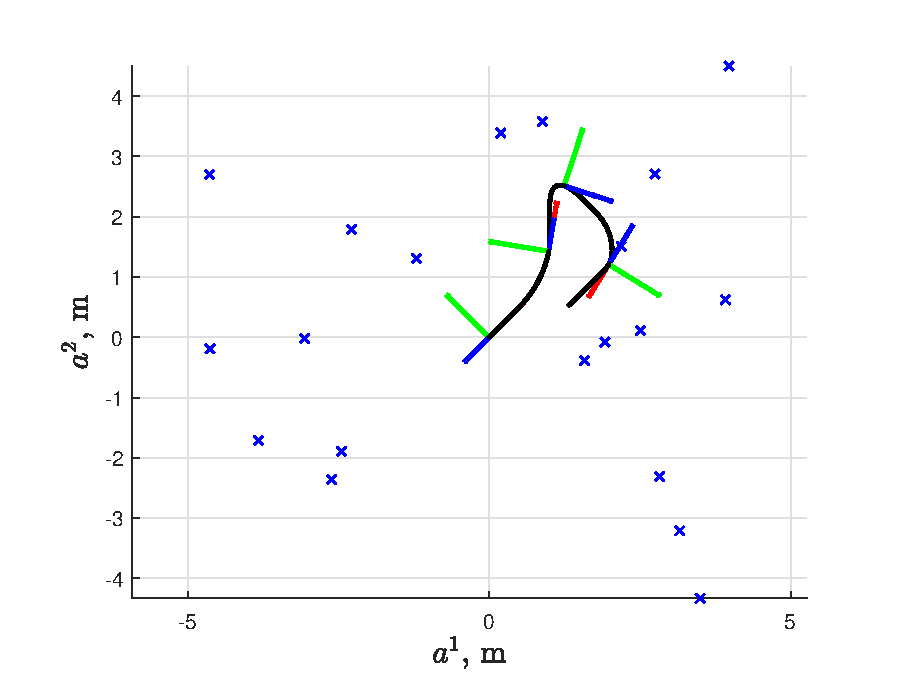
\includegraphics[width=\textwidth]{figs/batch/traj_xy.eps} 
        \end{subfigure}
        \hfill
        \begin{subfigure}[b]{0.495\textwidth}  
            \centering 
            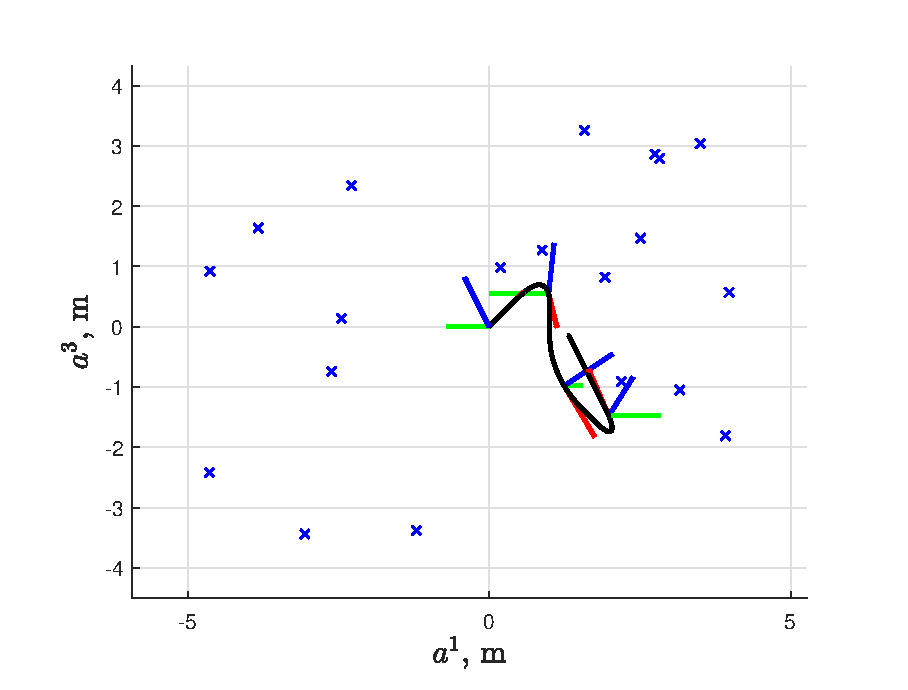
\includegraphics[width=\textwidth]{figs/batch/traj_xz.eps} 
        \end{subfigure}
        \vskip\baselineskip
        \begin{subfigure}[b]{0.495\textwidth}   
            \centering 
            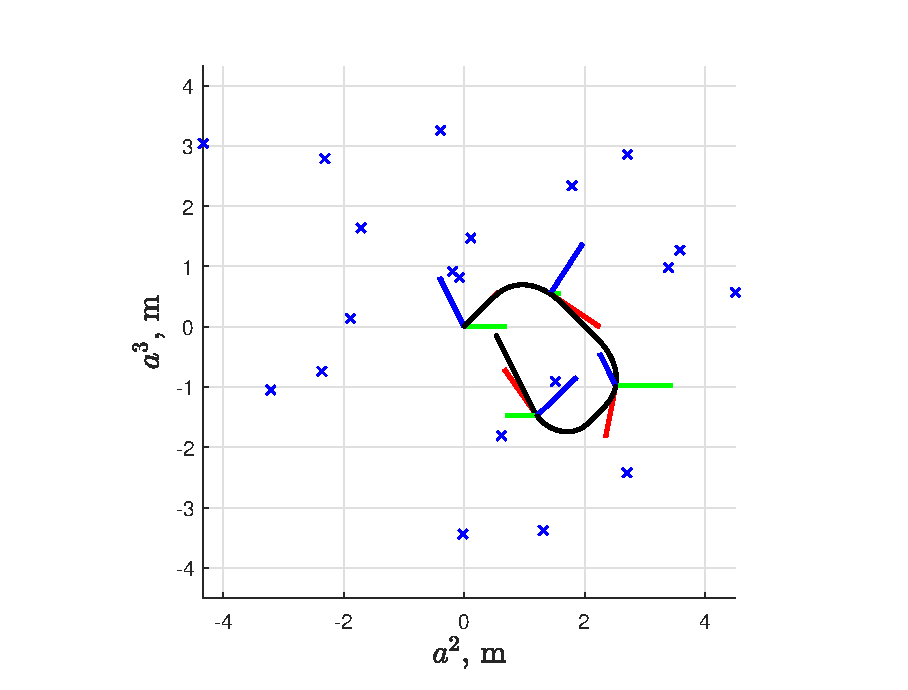
\includegraphics[width=\textwidth]{figs/batch/traj_yz.eps}  
        \end{subfigure}
        \hfill
        \begin{subfigure}[b]{0.495\textwidth}   
            \centering 
            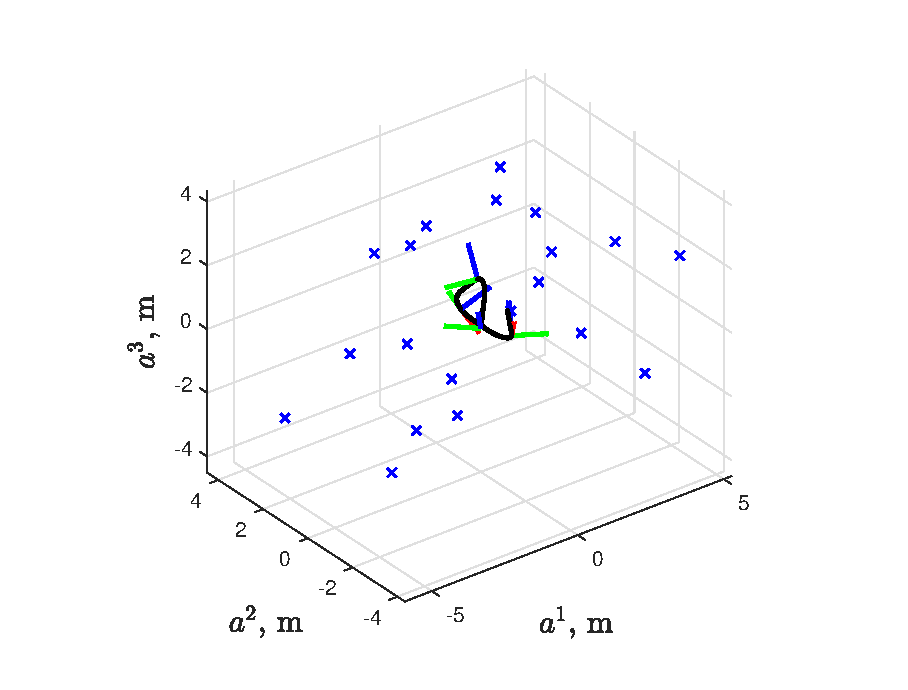
\includegraphics[width=\textwidth]{figs/batch/traj.eps} 
        \end{subfigure} 
	\caption[Trajectory used in simulations.]{Trajectory used in simulations. The blue markers represent the landmarks, the trajectory is shown in black, and a triad is used to show the orientation at various times during the trajectory.}
	\label{fig:batch_traj}
\end{figure}

\begin{table}[]
\centering
\begin{tabular}{|l|l|l|l|l|l|}
\hline
Trial                                            & $\sigma_k^1$ \si{\radian}          & $\sigma_k^2$ \si{m/s} & $\sigma_k^3$ \si{rad/s^2} & $\sigma_k^4$ \si{m/s^2} & $\sigma_{k,j}$ \si{m}      \\ \hhline{|=|=|=|=|=|=|}
\multicolumn{1}{|l|}{Rate Gyro Noise}            & \multicolumn{1}{l|}{0.05 to 1} & \multicolumn{1}{l|}{0.05}     & \multicolumn{1}{l|}{0.005} & \multicolumn{1}{l|}{0.005} & \multicolumn{1}{l|}{0.05}     \\ \hline
\multicolumn{1}{|l|}{Accelerometer Noise}  & \multicolumn{1}{l|}{0.05} & \multicolumn{1}{l|}{0.05 to 1}     & \multicolumn{1}{l|}{0.001} & \multicolumn{1}{l|}{0.005} & \multicolumn{1}{l|}{0.05}     \\ \hline
\multicolumn{1}{|l|}{Rate Gyro Bias Noise}  & \multicolumn{1}{l|}{0.05} & \multicolumn{1}{l|}{0.05}     & \multicolumn{1}{l|}{0 to 0.1} & \multicolumn{1}{l|}{0.005} & \multicolumn{1}{l|}{0.05}     \\ \hline
\multicolumn{1}{|l|}{Accelerometer Bias Noise} & \multicolumn{1}{l|}{0.05} & \multicolumn{1}{l|}{0.05}     & \multicolumn{1}{l|}{0.005} & \multicolumn{1}{l|}{0 to 0.1} & \multicolumn{1}{l|}{0.05}     \\ \hline
\multicolumn{1}{|l|}{Landmark Sensor Noise} & \multicolumn{1}{l|}{0.05} & \multicolumn{1}{l|}{0.05}     & \multicolumn{1}{l|}{0.005} & \multicolumn{1}{l|}{0.005} & \multicolumn{1}{l|}{0.05 to 1}     \\ \hline
\end{tabular}
\caption{Standard deviation of the noise injected into each measurement for each trial.}
\label{tab:se3_batch}
\end{table}

The results are presented in Figures~\ref{fig:batch_gyro}~to~\ref{fig:batch_landmark}. The main takeaway is that, generally, the six different approaches provide similar results. In particular, there is no discernible difference between using the invariant formulations of the measurement error (Approaches 4, 5, and 6) as opposed to their standard counterparts (Approaches 1, 2, and 3). The results from Approaches 1, 2, 4, and 5 are similar to such an extent that they are often indistinguishable when they are overlaid. Furthermore, the impact of reducing the state dependence of the Jacobians is unclear. After multiple iterations of the nonlinear least squares solver, the operating trajectory begins approaching the truth trajectory. Thus, assuming the solver converges to the optimal solution, the Jacobians become more and more accurate. The advantage of state-independent Jacobians is most notable in situations when the Jacobians are normally inaccurate, which isn't the case here. In addition, the error definitions used to derive the Jacobians in Approaches 3 and 6 simply shift the state dependence from $\mbf{F}_k^1$ to weighting matrix $\mbf{W}_{u,k}$. Some additional observations are as follows.

\begin{itemize}
	\item Increasing the magnitude of the standard deviation of the noise in the gyro had the largest impact on the results, as seen in Figure~\ref{fig:batch_gyro}. While Approaches 2 and 5 have a lower mean RMSE over a wide range of noise magnitudes, these formulations converge much slower than the other approaches. In the end, the left-invariant error definition using the type 1 Jacobians performed best when the noise level was increased.
	\item In general, a measurement-dependent Jacobian should be avoided when there is a lot of noise in the measurement, as it increases greatly the amount of steps needed to converge
	\item The right-invariant approaches show improved performance when there is significant noise in the landmark sensor and the accelerometer.
\end{itemize}

\begin{figure}
	\centering
	\begin{subfigure}[b]{0.5\textwidth}
		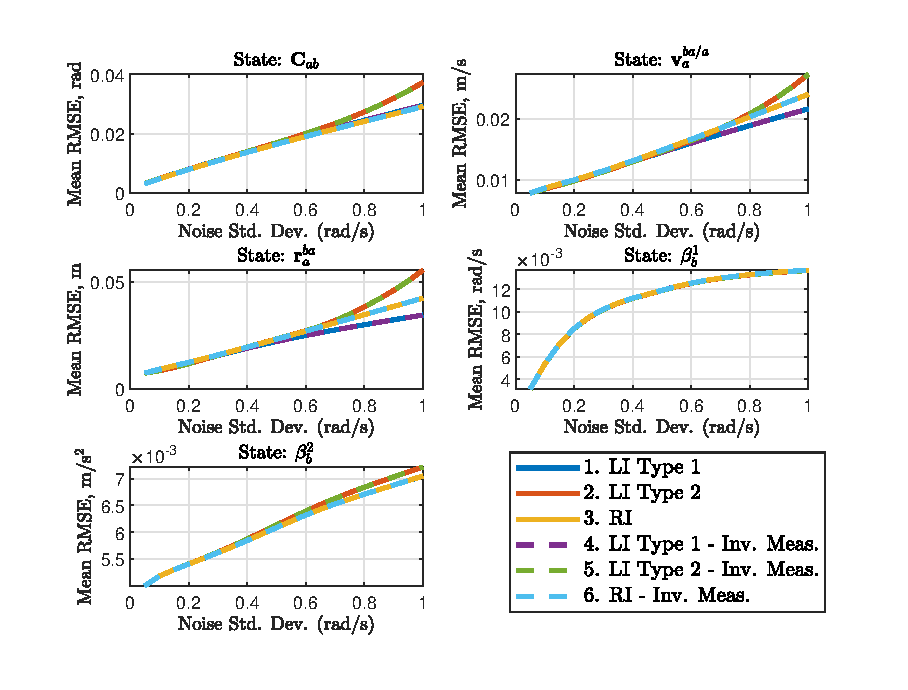
\includegraphics[width=\textwidth]{figs/batch/gyro_rmse.eps}
		\caption{Mean RMSE for each state.}
	\end{subfigure}
	~
	\begin{subfigure}[b]{0.5\textwidth}
		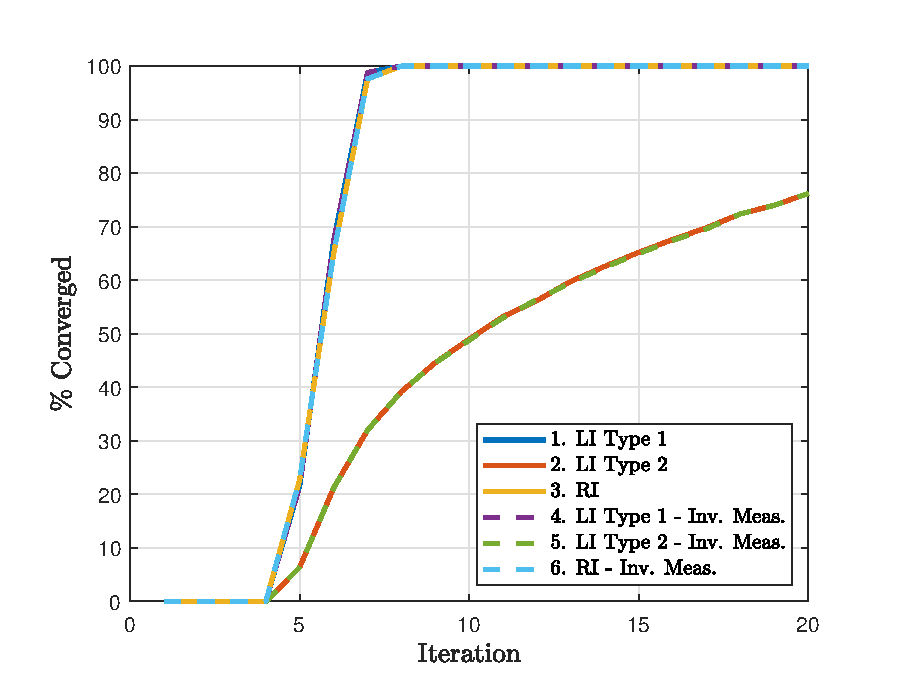
\includegraphics[width=\textwidth]{figs/batch/gyro_perc.eps}
		\caption{Percentage of trials that have converged at each GN iteration.}
	\end{subfigure}
	\caption[Results comparing batch SLAM approaches varying rate gyro noise.]{Results of 25 Monte Carlo trials comparing the various batch SLAM approaches, where the noise in the rate gyro was varied.}
	\label{fig:batch_gyro}
\end{figure}

\begin{figure}
	\centering
	\begin{subfigure}[b]{0.5\textwidth}
		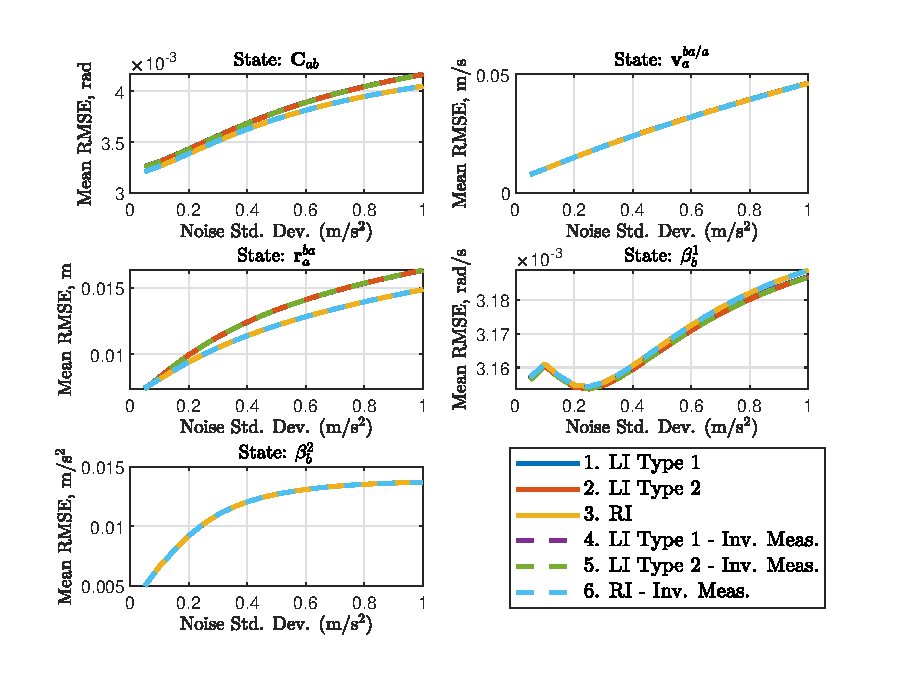
\includegraphics[width=\textwidth]{figs/batch/accel_rmse.eps}
		\caption{Mean RMSE for each state.}
	\end{subfigure}
	~
	\begin{subfigure}[b]{0.5\textwidth}
		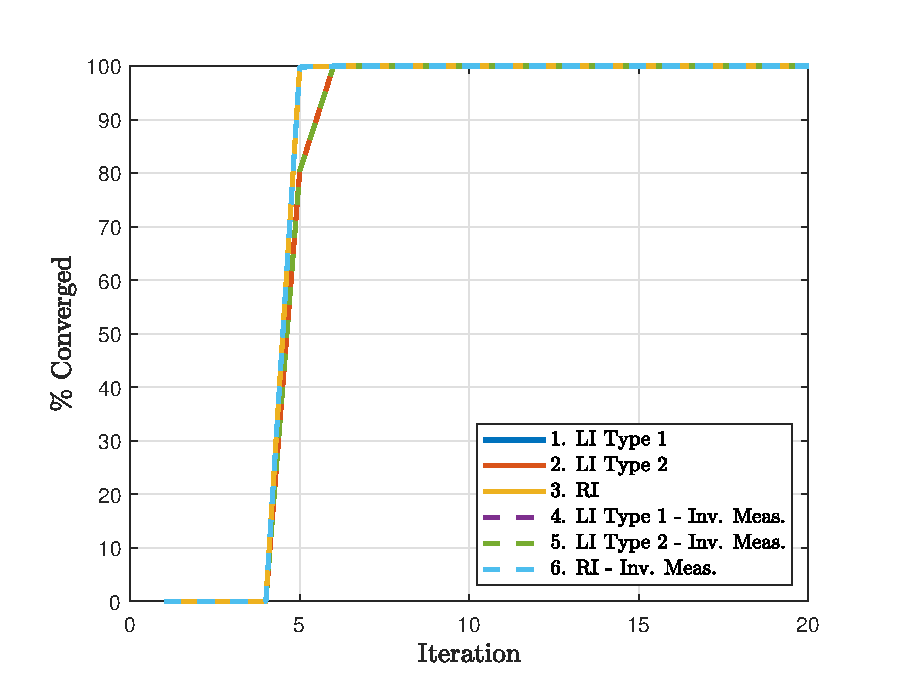
\includegraphics[width=\textwidth]{figs/batch/accel_perc.eps}
		\caption{Percentage of trials that have converged at each GN iteration.}
	\end{subfigure}
	\caption[Results comparing batch SLAM approaches varying zccelerometer noise.]{Results of 25 Monte Carlo trials comparing the various batch SLAM approaches, where the noise in the accelerometer was varied.}
	\label{fig:batch_accel}
\end{figure}  

\begin{figure}
	\centering
	\begin{subfigure}[b]{0.5\textwidth}
		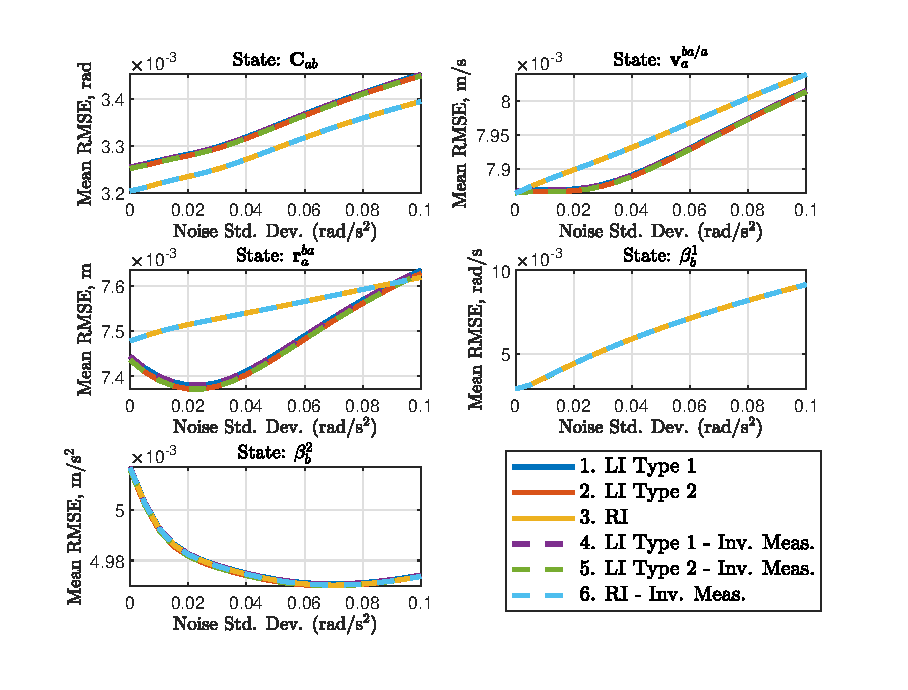
\includegraphics[width=\textwidth]{figs/batch/gyro_bias_rmse.eps}
		\caption{Mean RMSE for each state.}
	\end{subfigure}
	~
	\begin{subfigure}[b]{0.5\textwidth}
		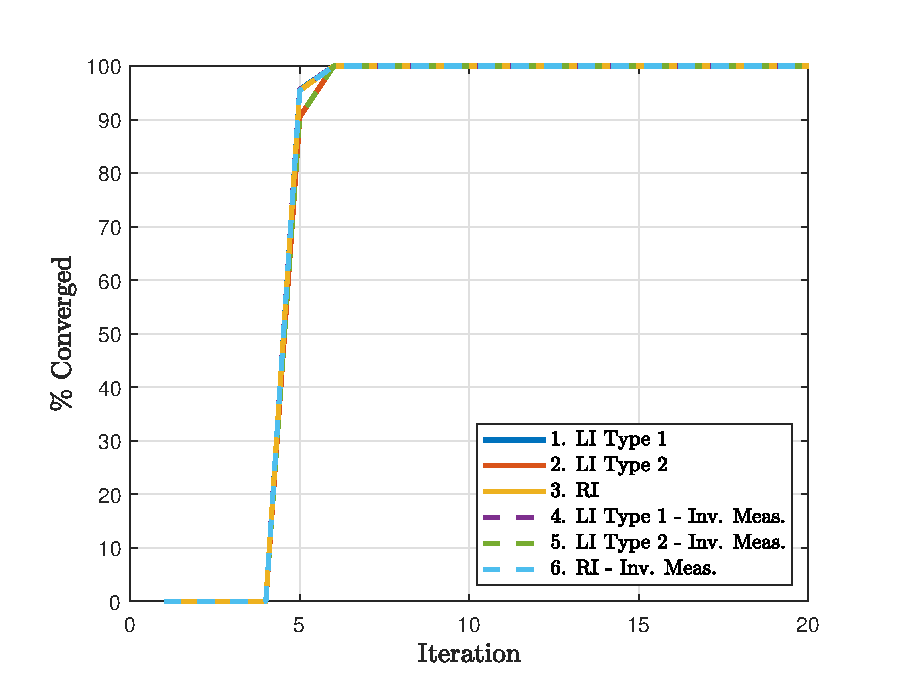
\includegraphics[width=\textwidth]{figs/batch/gyro_bias_perc.eps}
		\caption{Percentage of trials that have converged at each GN iteration.}
	\end{subfigure}
	\caption[Results comparing batch SLAM approaches vvarying rate gyro bias noise.]{Results of 25 Monte Carlo trials comparing the various batch SLAM approaches, where the noise in the gyro bias was varied.}
	\label{fig:batch_gyro_bias}
\end{figure} 


\begin{figure}
	\centering
	\begin{subfigure}[b]{0.5\textwidth}
		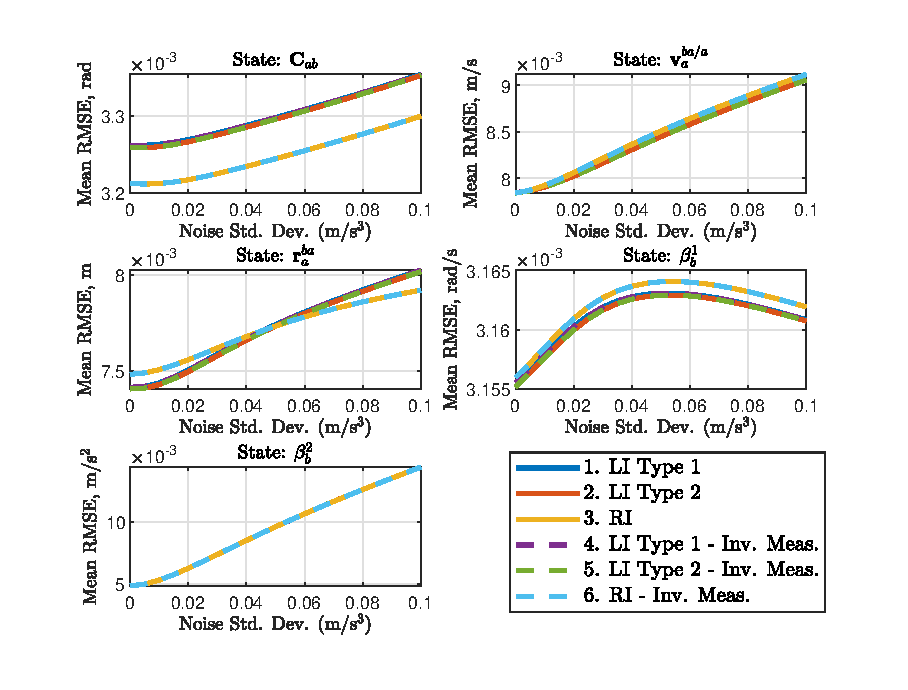
\includegraphics[width=\textwidth]{figs/batch/accel_bias_rmse.eps}
		\caption{Mean RMSE for each state.}
	\end{subfigure}
	~
	\begin{subfigure}[b]{0.5\textwidth}
		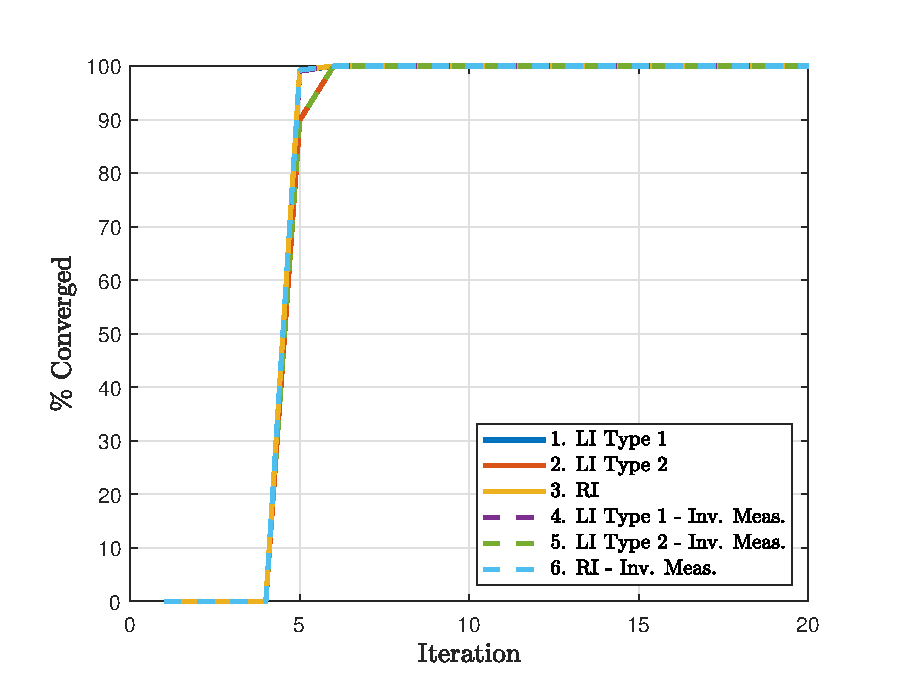
\includegraphics[width=\textwidth]{figs/batch/accel_bias_perc.eps}
		\caption{Percentage of trials that have converged at each GN iteration.}
	\end{subfigure}
	\caption[Results comparing batch SLAM approaches vvarying accelerometer bias noise.]{Results of 25 Monte Carlo trials comparing the various batch SLAM approaches, where the noise in the accelerometer bias was varied.}
	\label{fig:batch_accel_bias}
\end{figure} 

\begin{figure}
	\centering
	\begin{subfigure}[b]{0.5\textwidth}
		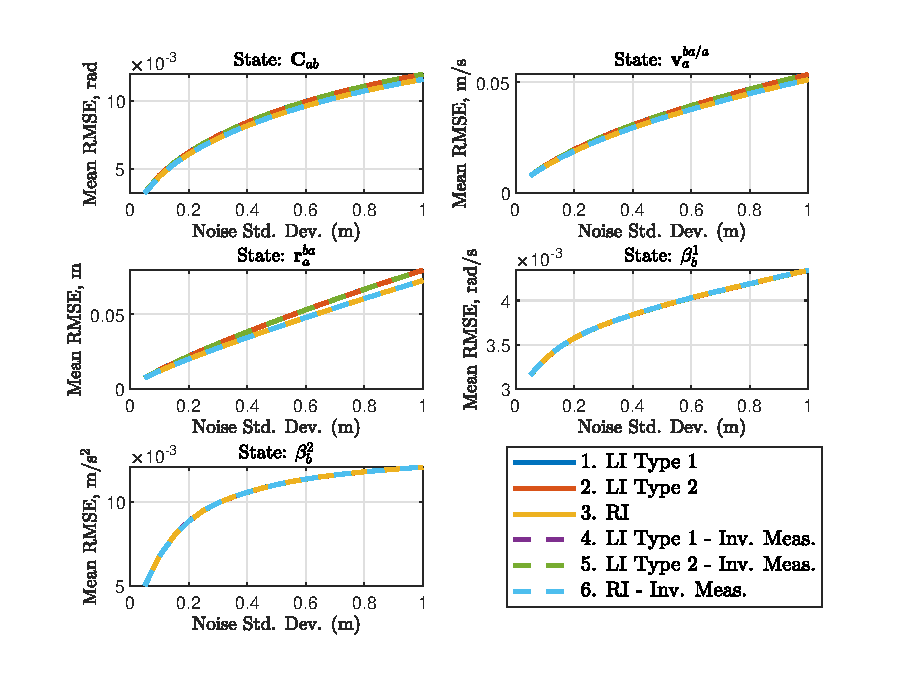
\includegraphics[width=\textwidth]{figs/batch/landmark_rmse.eps}
		\caption{Mean RMSE for each state.}
	\end{subfigure}
	~
	\begin{subfigure}[b]{0.5\textwidth}
		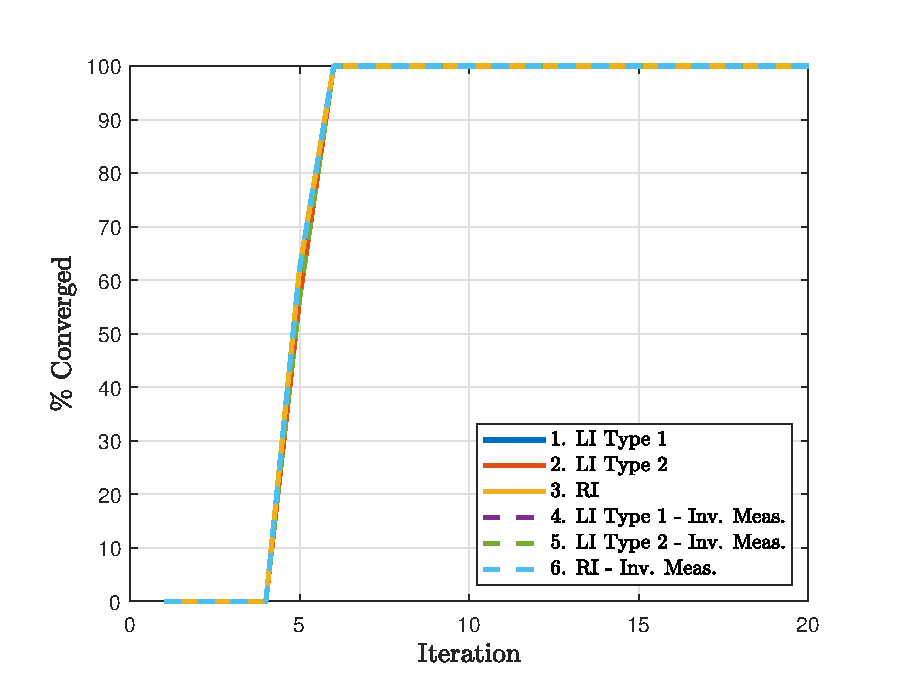
\includegraphics[width=\textwidth]{figs/batch/landmark_perc.eps}
		\caption{Percentage of trials that have converged at each GN iteration.}
	\end{subfigure}
	\caption[Results comparing batch SLAM approaches vvarying landmark sensor noise.]{Results of 25 Monte Carlo trials comparing the various batch SLAM approaches, where the noise in the landmark sensor was varied.}
	\label{fig:batch_landmark}
\end{figure}  